\chapter{呼吸困难}

呼吸困难是指患者主观上有空气不足或呼吸费力的感觉,而客观上表现为呼吸频率、深度(如呼吸速而浅或慢而深)和节律的改变。患者用力呼吸,可见辅助呼吸肌参与呼吸运动,严重者可呈端坐呼吸及发绀。

根据主要的发病机制,可将呼吸困难区分为下列五种基本类型。能引起呼吸困难的疾病繁多,见表\ref{tab3-1}。

\begin{table}[htbp]
\centering
\caption{呼吸困难疾病的分类}
\label{tab3-1}
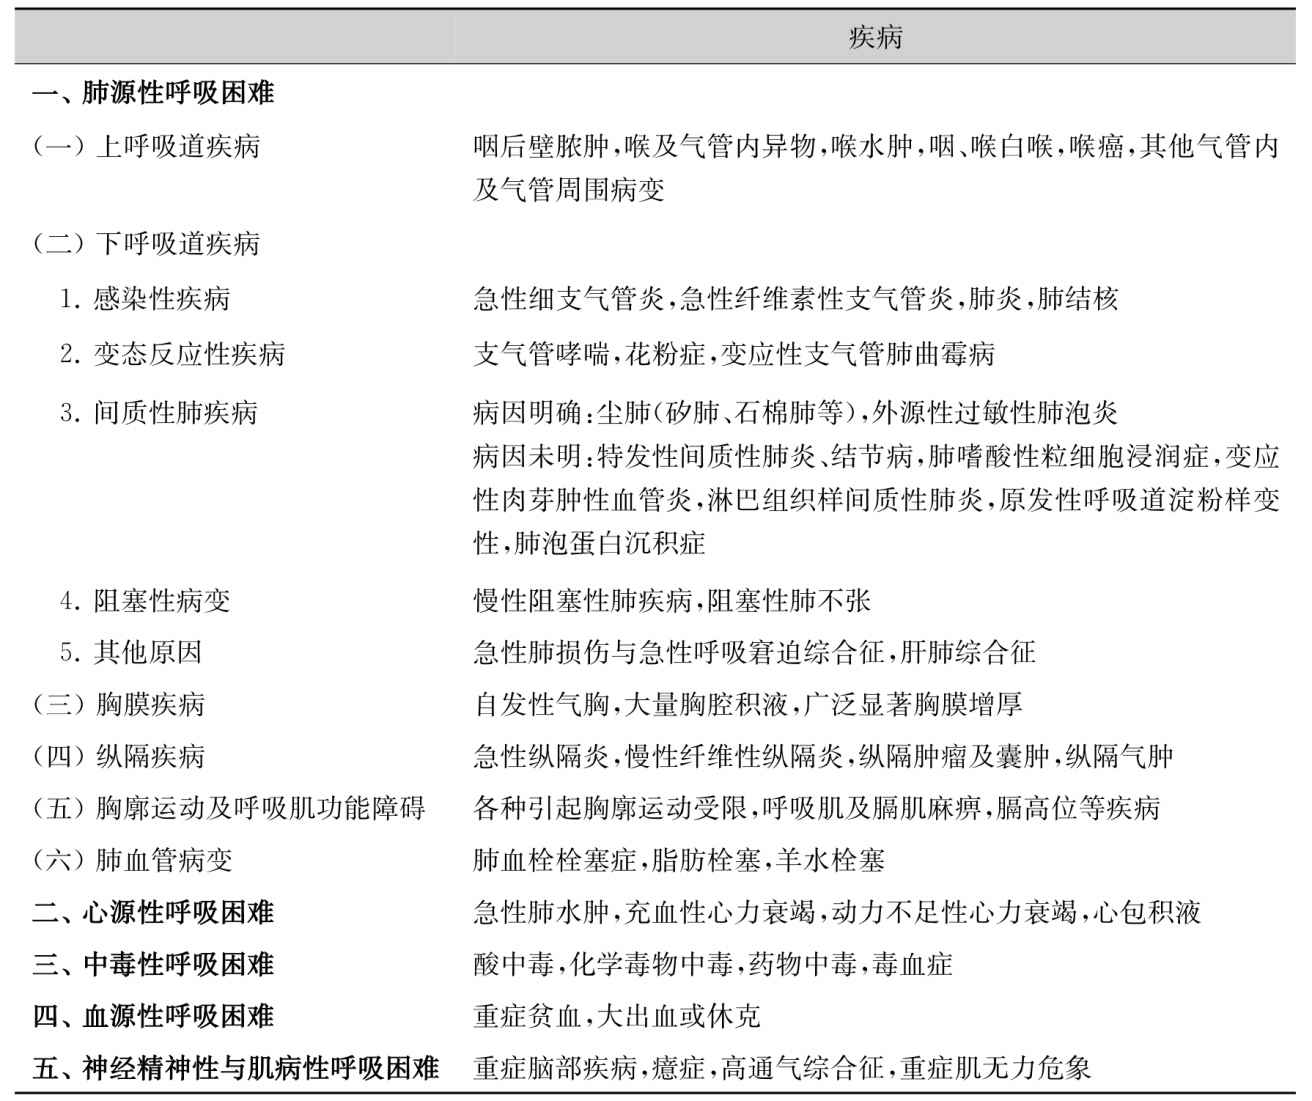
\includegraphics[width=5.95833in,height=5in]{./images/Image00032.jpg}
\end{table}

根据呼吸困难发生的缓急和伴随症状,可对呼吸困难作出初步的鉴别诊断:

\section{【急性发生的呼吸困难】}

1.时间超过1~2小时,伴有喘息者 支气管哮喘(病史可参考)、左心功能衰竭(心肌梗死、瓣膜病等)。

2.时间超过数小时/数天,伴有发热,有痰或无痰者 肺炎、急性支气管炎、急性胸膜炎、急性化脓性纵隔炎、急性心包炎等疾病。

3.高通气伴有代谢性酸中毒者 须考虑肾衰竭、糖尿病酮症酸中毒;有中毒者多为水杨酸盐、甲醇等。高通气综合征多为无心肺疾病的年轻女性。

4.呼吸困难同时伴有胸痛者 多为气胸(有气管移位)、肺栓塞(多有下肢静脉血栓,可有休克)、大叶性肺炎、急性心肌梗死、急性心包炎、急性胸膜炎、气道异物等。

5.产妇破水后突然出现呼吸困难、发绀、休克,应考虑为肺羊水栓塞症。长骨骨折后发生呼吸困难,须考虑肺脂肪栓塞。胸、腹大手术后突发呼吸困难,须考虑胸腔积液或肺不张。

\section{【慢性发生的呼吸困难】}

1.伴有胸膜炎性胸痛应注意胸腔积液、叶性肺不张、气胸、肺炎和肺栓塞等。

2.伴有大量脓性痰者多为支气管扩张,小量脓性痰可见于慢性支气管炎、支气管哮喘和肺炎。大量粉红色泡沫痰则见于急性左心功能不全,但也可见于肺泡细胞癌。

3.伴有咯血者如胸部X线检查显示中央气道异常可能是肺癌,胸部X线检查正常则可能为肺栓塞或肺血管炎(如Goodpasture综合征、多发性动脉炎)。

4.伴有全身衰弱者应注意神经肌肉疾病,如重症肌无力和运动神经元疾病。

\section{【如何评价呼吸困难】}

\subsection{(一)病史}

心、肺、胃肠病及肾脏病史,以往气喘发作史及诊疗经过,内因性与外因性中毒,职业性粉尘或异物吸入史,过敏病史,用药史,高原居留史。

病史询问应了解下列问题:①呼吸困难是突然发生还是逐渐发生?②患者的年龄,以及症状缓解和恶化的特点?③是休息还是活动时出现呼吸困难?④出现呼吸困难症状时的活动程度如何?临床上常用改良的呼吸困难分级量表(modified
Medical Research Council dyspnoea
scale,mMRC)评估呼吸困难程度,特别适用于慢性支气管炎和慢性阻塞性肺疾病患者。mMRC分为0~4级共5个级别,级别越高,患者呼吸困难越重:其中0级表示患者仅在费力运动时出现呼吸困难;4级表示患者因严重呼吸困难不能离开家,或在脱/穿衣服时出现呼吸困难。急性呼吸困难常常导致严重的后果,需要立刻评估和治疗(表\ref{tab3-2})。

\begin{table}[htbp]
\centering
\caption{呼吸困难程度}
\label{tab3-2}
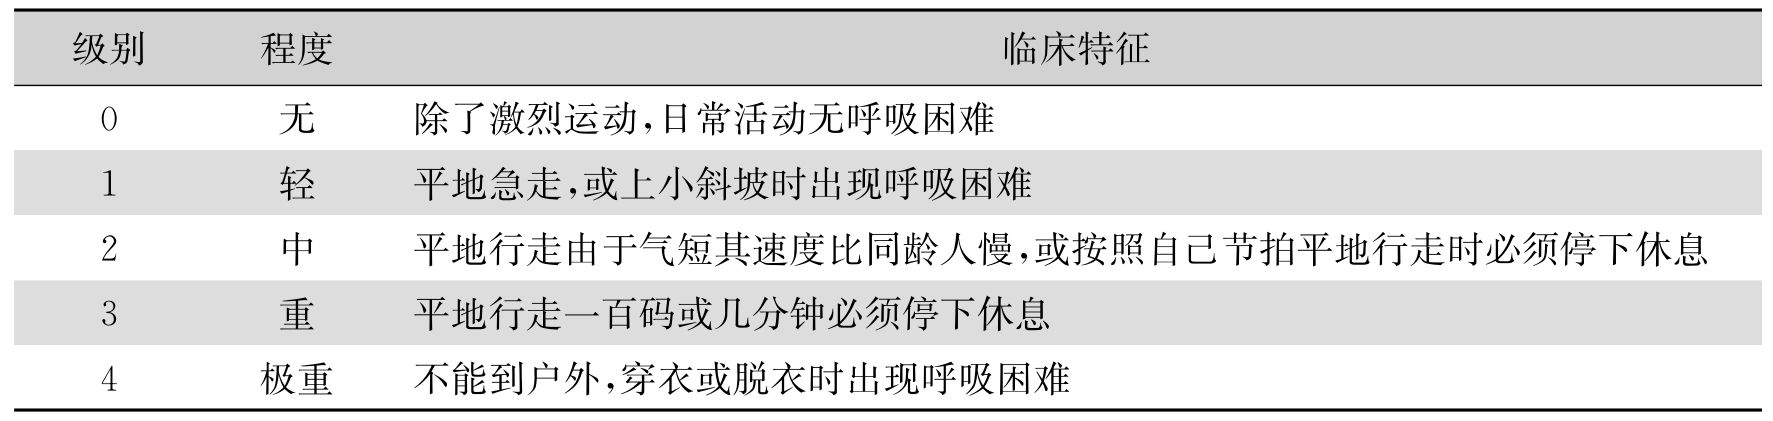
\includegraphics[width=5.90625in,height=1.39583in]{./images/Image00033.jpg}
\end{table}

\subsection{(二)体检}

咽、喉与胸部体征,肝脾大,腹水、水肿。肺部是体检的重点。另外还需评估患者的心脏情况,排除心脏疾病。

\subsection{(三)化验检查}

血象,嗜酸性粒细胞计数,有指征时作血尿素氮、血糖测定、动脉血气分析与酸碱度测定、痰检查(包括痰涂片找抗酸杆菌、痰培养和痰的细胞学分析等)。

\subsection{(四)器械检查}

X线胸部透视或(及)摄片;有指征时作静脉压测定、血循环时间测定、心电图描记、肺功能检查、放射性核素肺扫描、CT、纤维支气管镜检查、肺血管造影等。

\protect\hypertarget{text00044.html}{}{}

\section{7 肺源性呼吸困难}

广义的肺源性呼吸困难是由于呼吸器官(包括上呼吸道、支气管、肺、胸膜)病变、纵隔病变、胸廓运动以及呼吸肌功能障碍等所致,可分为下列三种表现形式:

\subsection{(一)吸气性呼吸困难}

可见于急性咽后壁脓肿、喉水肿、喉痉挛、喉及气管内异物、咽、喉白喉、喉癌、气管息肉、气管肿瘤、气管受压(气管周围脓肿、甲状腺肿瘤或甲状腺术后出血等)等疾病。由于喉、气管与大支气管狭窄与阻塞所致。

\subsection{(二)呼气性呼吸困难}

可见于急性细支气管炎、支气管哮喘、慢性阻塞性肺气肿、外源性过敏性肺泡炎等疾病。由于肺组织病变如弹性减弱及小支气管痉挛、狭窄所致。

\subsection{(三)混合性呼吸困难}

可见于慢性阻塞性肺气肿合并肺部感染,大量胸腔积液,自发性气胸,广泛性肺实质性病变如急性粟粒型肺结核,大叶性肺炎与支气管肺炎,大片肺不张以及急性肺水肿等疾病。由于肺呼吸面积减少所致。

\protect\hypertarget{text00045.html}{}{}

\subsection{7.1 上呼吸道疾病}

喉与气管病变所致的呼吸困难,其特点是吸气性呼吸困难,吸气时带有喘鸣音,常伴有声嘶与失音,呼吸深大但不快,吸气时呼吸肌运动加强,并可出现胸骨上窝、锁骨上窝与肋间的凹陷现象。

\subsubsection{一、咽后壁脓肿}

咽后壁脓肿多见于小儿,较少见于成人。年龄愈小或脓肿愈近喉部,则呼吸困难愈明显,并有喘鸣音、吞咽疼痛、吞咽困难。由咽后壁淋巴结化脓及异物损伤咽后壁所致的非特异性化脓性脓肿,其起病急骤,并有化脓感染的全身性症状;由结核菌引起的脓肿则呈慢性经过。

本病的诊断可根据:①咽部视诊可发现咽后壁红肿,轻触脓肿部位有波动感;②颈椎侧位X线摄片可显示咽后壁隆起的软组织肿胀;③结核性者可有颈椎结核的X线征。

\subsubsection{二、喉及气管内异物}

喉及气管内异物绝大多数发生于5岁以下的小儿及昏迷患者。异物卡住喉腔可引起高度呼吸困难以致窒息。异物进入气管内则引起刺激性咳嗽,以后停留在恰能容下其大小的部位,引起阻塞性肺气肿、肺不张与局灶性感染。异物多为食物、骨头、果核、小金属物和笔套等;在昏迷患者则为呕吐物、假牙等。胸部X线检查,可发现不透X线的异物影、局限性肺气肿、肺不张或阻塞性肺炎。喉镜或纤维支气管镜检查有助于观察异物的大小、性状与所在位置,并可在直视下取出异物。

\subsubsection{三、喉水肿}

喉水肿多急骤起病,水肿波及整个黏膜下层时,病情较轻者有喉内异物感、吞咽梗阻感、干咳、声嘶,严重者则引起呼吸困难。如声门或声门下区水肿,可迅速产生致命的喉梗阻。

引起喉水肿的原因可分为感染性和非感染性二类。感染性者,如化脓性咽喉炎、喉结核、喉部脓肿;非感染性者,如血管神经性水肿、药物过敏(如碘剂、乙酰水杨酸等)、喉部外伤、异物损伤及刺激(如气管插管)、高热蒸气或强烈化学气体(如氯气、光气、氨气、二氧化硫气等)刺激、腐蚀剂(如高浓度高锰酸钾溶液)刺激等。

血管神经性水肿所致的喉水肿,多有身体其他部位过敏征象出现,且有多次反复发作史;药物过敏性喉水肿有服用药物史;喉部化脓性炎症有明显感染症状。

\subsubsection{四、咽、喉白喉}

咽白喉约占白喉患者的80\%,病情轻者有咽痛、低中度发热,无明显全身中毒症状。重型和极重型患者有高热、头痛、面色苍白、呼吸急促、呼吸困难、烦躁不安、脉细速等全身中毒症状,并可出现中毒性心肌炎、周围神经麻痹,甚至中毒性休克。体检咽部充血,扁桃体肿大,咽部有点状或小片状灰白色假膜形成,不易剥离。有些患者咽部假膜范围广且厚,可呈污秽的黑灰色,有腐败口臭,扁桃体及咽部高度肿胀,可有坏死或溃疡,可合并其他细菌感染;颈部淋巴结肿大,周围软组织水肿,可蔓延至胸部,状似“牛颈”。

喉白喉约占白喉患者的20\%,多见于小儿,多数由咽白喉蔓延而来,起病略缓。白喉假膜和喉局部炎症、水肿引起气道狭窄,出现喉痛、吞咽困难、“犬吠”样咳嗽、声嘶、吸气性呼吸困难与喘鸣音,以及全身中毒症状,严重喉梗阻者吸气时出现“三凹征”。假膜涂拭物涂片染色或培养检查发现白喉杆菌而确诊。

喉白喉须与急性喉炎区别。小儿有发热、“犬吠”样咳嗽、声音嘶哑、吸气性呼吸困难者,应考虑喉白喉与急性喉炎。后者起病急骤、高热、呼吸困难常呈昼轻夜重,喉镜检查无灰白色假膜发现。

\subsubsection{五、急性会厌炎}

急性会厌炎又称急性声门上喉炎,好发于成人,可分两种临床类型,即渐进型(缓慢型)和速发型(暴发型)。咽部疼痛和吞咽困难是成人急性会厌炎最常见的症状。本病初起常隐匿,仅有轻微咽痛,数小时后病情突然加重,咽痛难忍,吞咽困难,喘鸣、呼吸困难。一些患者常于夜间熟睡中突然痛醒而急诊就医。该病速发型以起病突然,来势凶险为特征,呼吸困难多在起病3~12小时内发生,可引起喉阻塞而窒息、死亡,是耳鼻咽喉科临床急重症之一。

\subsubsection{六、喉 癌}

喉癌多见于中年以上(尤以40~60岁)的男性。男女发病比例为7~10∶1。喉癌初期发展较慢,逐渐出现吞咽不适、喉部异物感、声嘶和吞咽痛,后期出现呼吸困难。进行性喉癌常有呼吸困难,声门下区癌尤为明显,声门上区癌则较轻;此外尚有声嘶、失音、咳血痰等。癌转移则引起颈部淋巴结肿大。凡年逾40岁,声嘶超过6周的喉部不适患者,须注意喉癌的可能性,应做喉镜检查。如为喉癌,可显示肿瘤轮廓、软组织间隙变形、软骨移位等。

\subsubsection{七、其他气管内及气管周围病变}

气管内病变如气管息肉、肿瘤、淀粉样变性,气管韦格纳肉芽肿,喉气管复发性多软骨膜炎;气管的物理和化学性损伤;气管手术、外伤后肉芽、瘢痕组织形成;气管周围脓肿,甲状腺、颈段食管肿瘤,甲状腺术后出血等造成的气管外压迫等亦可引起呼吸困难,临床上应相应辨别及处理。

国内曾报道一组11例罕见的颈段气管相关病变所致的呼吸困难,其中气管内病变4例(息肉1例,韦格纳肉芽肿3例),气管周围病变4例(脓肿2例,甲状腺癌2例),气管本身病变3例,为复发性多软骨膜炎。

\protect\hypertarget{text00046.html}{}{}

\subsection{7.2 下呼吸道疾病}

\subsubsection{7.2.1 感染性疾病}

\paragraph{一、急性细支气管炎}

急性细支气管炎多见于小儿,特别是2岁以内的婴幼儿,偶见于年长儿童和成人。呼吸道合胞病毒是其最常见的病原体,其病理基础是呼吸道病毒感染所致的细支气管痉挛、炎症与水肿。临床上以呼吸窘迫、喘吼、呼气阻塞和缺氧为特征,感染控制后症状也随之消退。与支气管哮喘的鉴别是:①气喘发作与缓解均较缓慢,不如支气管哮喘发作的突然与缓解的迅速;②常有呼吸道感染症状,发作时肺部除干性啰音外,湿性啰音也相当明显;③痰往往呈脓性,镜检有大量中性粒细胞,而支气管哮喘时则有大量嗜酸性粒细胞,血象中性粒细胞增多;④对支气管舒张剂的反应不及支气管哮喘。

\paragraph{二、急性纤维素性支气管炎}

本病少见,主要表现为咳嗽、胸闷、呼吸困难、发绀、发热以及反复咯血等,其诊断依靠从患者咳出物中找到树枝状支气管样管型和咳出物病理检查主要为纤维素样物质而诊断。(参见第14节之“十”)。

\paragraph{三、肺 炎}

包括病毒性肺炎(如流感病毒性肺炎、严重急性呼吸综合征)、衣原体肺炎(如肺炎衣原体肺炎、鹦鹉热衣原体肺炎)、恙虫病立克次体肺炎,以及各种细菌性肺炎(如肺炎链球菌肺炎、肺炎克雷伯杆菌肺炎、金黄色葡萄球菌性肺炎)等(参见第3.1节)。

\paragraph{四、肺结核}

急性粟粒型肺结核、支气管结核、干酪样肺炎等均可引起呼吸困难。

\subsubsection{7.2.2 变态反应性疾病}

\paragraph{一、支气管哮喘}

支气管哮喘的主要症状是反复发作性的喘息、胸闷、呼吸困难或咳嗽,多数患者可自行缓解,或给予支气管舒张药治疗而缓解。诱因常为接触变应原、冷空气、物理化学性刺激、病毒性上呼吸道感染、运动等。有些患者可经年反复发作。发作时患者喘息、胸闷、呼吸困难或咳嗽,伴有双肺哮鸣音,重者有焦虑、烦躁、发绀、大汗淋漓,患者常取端坐体位。发作时间短者仅数分钟,长者达数小时,甚至数天。发作停止后,患者能自由活动,一如平时。患者痰液或血中嗜酸性粒细胞可增多。

此病的诊断可根据:①反复发作喘息、胸闷、呼吸困难或咳嗽,多有诱因;②发作时在双肺可闻及散在或弥漫性、以呼吸相为主的哮鸣音,呼气相延长;③症状可经治疗缓解或自行缓解;④临床表现不典型者应做支气管激发试验/运动试验、支气管舒张试验或测量昼夜呼气峰值流速(PEF)变异率,三项检查中至少一项阳性;⑤除外其他相似症状的疾病,如慢性支气管炎、阻塞性肺气肿、心源性哮喘、变态反应性肺浸润等。

心源性哮喘与支气管哮喘发作时,二者的症状颇相似。心源性哮喘有时被误诊为支气管哮喘,二者的鉴别可参考表\ref{tab3-3}。

\begin{table}[htbp]
\centering
\caption{支气管哮喘与心源性哮喘的鉴别}
\label{tab3-3}
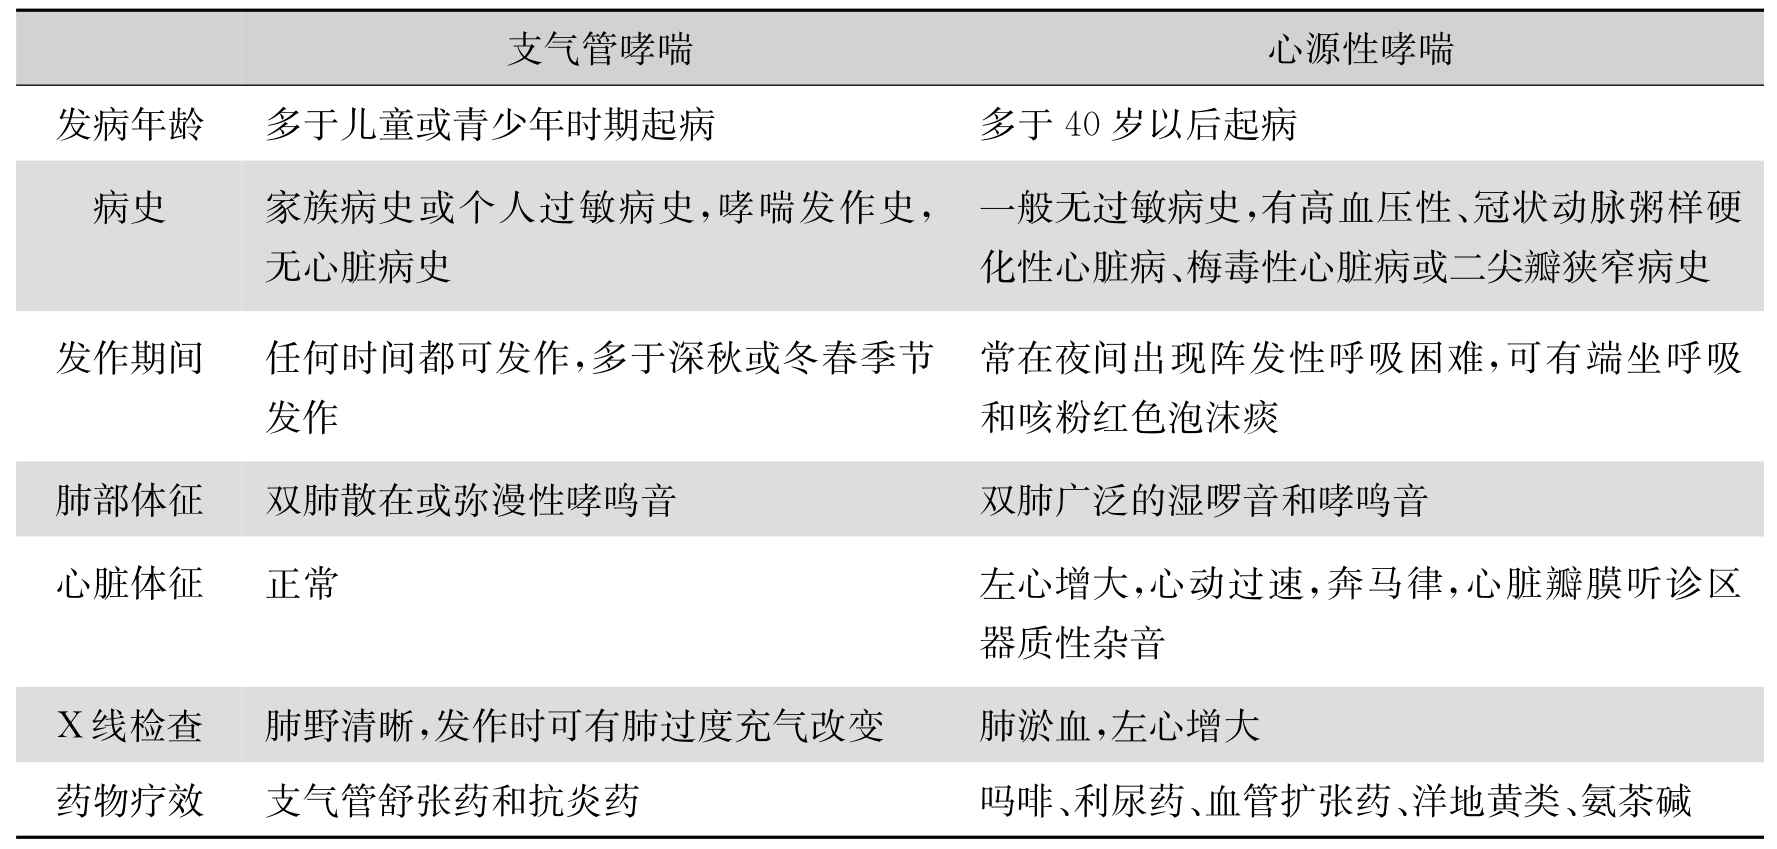
\includegraphics[width=5.91667in,height=2.82292in]{./images/Image00034.jpg}
\end{table}

\paragraph{二、职业性哮喘}

职业性哮喘近年有逐渐增多的趋势。哮喘发作与职业有关者统称职业性哮喘,诊断上应注意发病与职业上有害物质的关系。发病机制主要有:①职业接触物作为变应原,引起主要以IgE介导的速发型超敏反应;②职业有害物质引起药理介质的释放失调;③职业有害物质的非特异刺激反应,其中超敏反应起主导作用。

职业性哮喘的临床特点是:①患者在就业前不存在哮喘;②就业以后发生哮喘(一般可有数月乃至数年的潜伏期);③患病后每从事有害作业时则引起哮喘发作,脱离工作环境或假期休息时则可自行缓解,但再接触后又可发作。

工作环境中的职业性致喘物有400多种,广泛分布于化工、染料、合成纤维、橡胶皮革、纺织、制药、油漆、塑料黏合剂、印刷、冶炼、农药、木材加工、粮食、家禽饲养、农作物种植等。诊断可根据职业史和上述哮喘的特点综合考虑,必要时可行职业变应原支气管激发试验。

\paragraph{三、花粉症}

对花粉过敏者吸入花粉有的可引起气喘。花粉症在我国分布颇广,多由于黄花蒿、臭蒿、艾蒿、茵陈蒿等蒿属植物花粉所引起。此病与支气管哮喘的主要不同点是:①此病发作于花粉散发季节,且多在清晨、晴朗有风之时;②患者常伴有过敏性上呼吸道炎的表现,如流清涕、打喷嚏、鼻塞、眼和鼻奇痒,少数患者可有荨麻疹;③鼻黏膜分泌物涂片检查可发现大量嗜酸性粒细胞。以花粉作鼻黏膜激发试验,阳性率较高,有诊断意义。但应注意有的患者合并有支气管哮喘。

\paragraph{四、变应性支气管肺曲霉病(allergic bronchopulmonary}
aspergillosis,ABPA)

多由烟曲霉引起的气道高反应性疾病。对曲霉过敏者吸入大量孢子后,阻塞小支气管,引起短暂的肺不张和喘息发作,亦可引起肺部反复游走性浸润。患者表现为呼吸困难、喘息、畏寒、发热、乏力、刺激性咳嗽、咳棕黄色脓痰,偶带血。痰中有大量嗜酸性粒细胞及曲霉丝,烟曲霉培养阳性。哮喘样发作为其突出的临床表现,一般解痉平喘药难以奏效,外周血嗜酸性粒细胞增多。典型X线胸片为上叶短暂性实变或不张,可发生于双侧。胸部HRCT呈“近端”或中央支气管囊状扩张及壁增厚征象。诊断标准见第3.1.7节。

\subsubsection{7.2.3 间质性肺疾病}

间质性肺疾病(ILD)是一组主要累及肺间质、肺泡及(或)细支气管的肺部弥漫性疾病,目前已包括200多个病种,按病因明确与否分为病因已明和病因未明两大类,各病种的发病机制有显著区别,但临床上均表现为渐进性劳力性呼吸困难,限制性通气功能障碍伴弥散功能降低,低氧血症。胸部影像学显示双肺弥漫性病变,晚期发展为弥漫性肺纤维化和蜂窝肺,导致呼吸衰竭。

\paragraph{一、尘 肺}

尘肺是在生产活动中长期吸入生产性粉尘所引起的肺间质纤维化疾病,常见有硅沉着病(矽肺)、煤工尘肺、石棉肺和慢性铍肺等,重症患者有呼吸困难症状,在肺功能不全后期更为明显(参见第29节)。

\subparagraph{(一)棉尘肺}

棉纺工人发生气喘发作,须考虑是否为棉尘肺。此病的特点是,罹患此病的棉纺工人在每星期日休息之后,星期一再接触棉尘时便出现胸闷、气急、咳嗽、咳痰(部分病例可带血)等症状,但无发热。轻者工作一二天后症状渐缓解,严重者可持续至脱离接触后仍有症状。此病与长期吸入较高浓度的棉尘(尤以用低级棉为原料及粗纺车间工作者较多罹患)有关,是以支气管痉挛为基本病变的过敏性疾病。此病的主要诊断根据:①有职业史及发作的特殊规律;②肺部X线征可表现为慢性支气管炎、肺气肿征,重症者可呈广泛性网织状阴影。

\subparagraph{(二)霉草尘肺}

此病乃因接触潮湿发霉的干草,吸入带有真菌及其孢子的霉草尘所引起,罹患者以农民为多。患者常在接触后2~3小时发生呛咳、胸闷,继而咳出白色泡沫状或黏液性痰,气喘,并常有乏力、畏寒、发热等全身症状,有时出现荨麻疹。听诊双肺有弥漫性哮鸣音。血中嗜酸性粒细胞增多。X线检查可发现肺部短暂性、炎症性片状阴影及支气管周围炎征象。

所谓甘蔗渣肺也是同类疾病,见于接触发霉甘蔗渣的人。

\subparagraph{(三)蘑菇肺}

本病为蘑菇培植者的过敏性肺泡炎,也可见于平菇培植者。本病开始时易被误诊为感冒或支气管炎,主要表现为咳嗽、咳痰、胸痛、胸闷、咽痛、低热等症状,重症者有气短或呼吸困难;可有皮疹与X线肺部阴影。痰及血中常有嗜酸性粒细胞增多。本病可区分为三种临床类型:①高热型,以高热为主要症状;②支气管炎型,以支气管炎症状为主;③轻型:临床症状轻微而X线胸片有异常。X线胸片大多呈弥漫性阴影,少数呈局限性阴影。

\paragraph{二、外源性过敏性肺泡炎}

多数为在工作场所吸入了植物性或动物性有机粉尘所引起,包括农民肺、棉尘肺、霉草尘肺、甘蔗渣肺、蘑菇肺、饲鸽者肺、湿化器和空调器肺、烟草工人肺、木工肺等数十种,发病机制目前尚未完全明确,但抗原-抗体复合物和T细胞介导的免疫反应是主要的发病机制,尤其后者更为重要。

临床特点:①患者发作的症状严重程度与机体对吸入抗原的免疫反应、粉尘的抗原性、接触强度、次数及持续时间有关,可为急性、亚急性或慢性发作。②急性发作者一般在吸入大量抗原4~8小时后发作,表现为呼吸困难、干咳、胸闷,可有畏寒寒战、高热、全身不适等症状,脱离粉尘接触后1~3天内症状自然消失,少数可持续1周左右;亚急性常由急性发展而来,症状可持续数日或数周;慢性者起病隐匿,咳嗽、呼吸困难等进行性加重,常因不能及时诊治或脱离有机粉尘环境而发展为慢性肺间质纤维化,导致慢性肺心病。③用特异性抗原溶液行吸入激发试验或抗原皮肤试验常阳性。

部分急性外源性过敏性肺泡炎患者在吸入抗原后可出现哮喘症状,应与支气管哮喘鉴别,参考表\ref{tab3-4}。

\begin{table}[htbp]
\centering
\caption{外源性过敏性肺泡炎与支气管哮喘的鉴别}
\label{tab3-4}
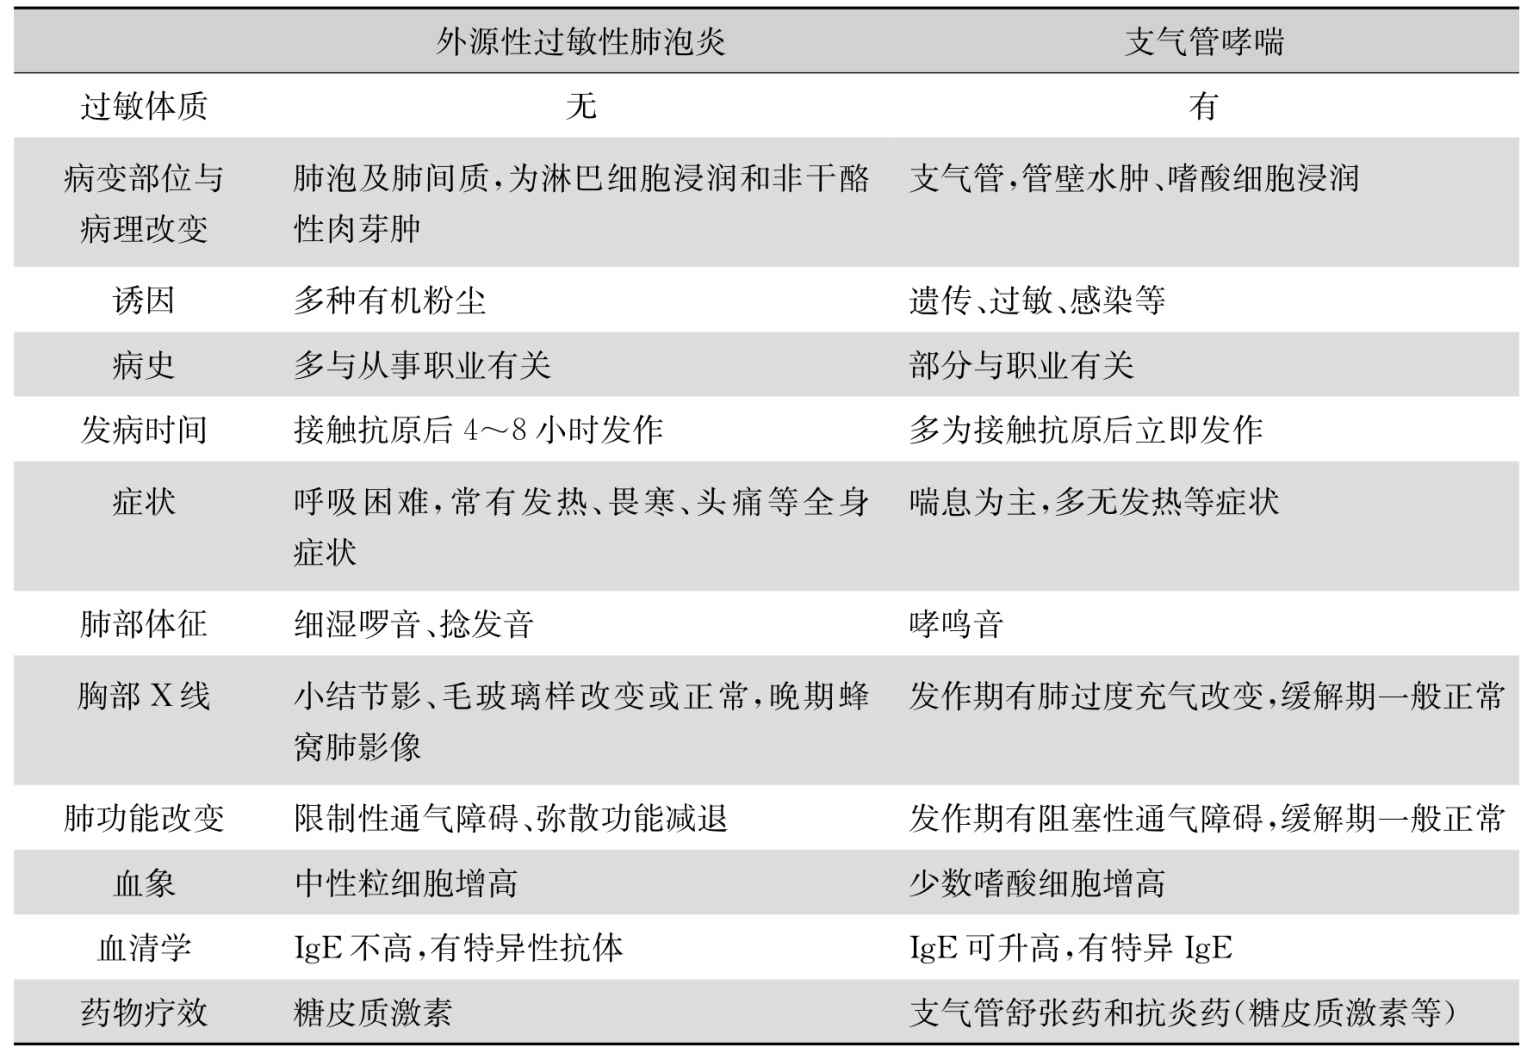
\includegraphics[width=5.90625in,height=4.09375in]{./images/Image00035.jpg}
\end{table}

\paragraph{三、特发性间质性肺炎}

特发性间质性肺炎(IIPs)是一组原因不明的肺间质性疾病,其分类与命名几经修改,目前的分类同时强调了临床-放射-病理诊断,包括了特发性肺纤维化(IPF)、非特异性间质性肺炎(NSIP)、隐源性机化性肺炎(COP)、急性间质性肺炎(AIP)、呼吸性细支气管炎间质性肺疾病(RBILD)、脱屑性间质性肺炎(DIP)、淋巴细胞性间质性肺炎(LIP)、特发性胸膜肺实质纤维弹性组织增生症(IPPF)和未分类特发性间质性肺炎(UCIIP)各自不同的实体疾病。这组疾病的临床表现非常相似,缺乏诊断特异性,但预后和治疗反应的差异性很大,故需要结合临床、放射学、肺生理功能、支气管肺泡灌洗和组织病理学等综合评估,才能明确最后诊断,并注意排除结缔组织疾病、药物、职业、感染等所致的继发性间质性肺疾病。

\subparagraph{(一)特发性肺纤维化}

特发性肺纤维化(IPF)是指原因不明并以普通型间质性肺炎(UIP)为特征性病理改变的一种慢性炎症性间质性肺疾病,占所有IIPs的60\%以上,主要表现为弥漫性肺泡炎、肺泡单位结构紊乱和肺纤维化。临床表现:①发病年龄多在中年以上,男∶女≈2∶1,儿童罕见;②起病隐袭,主要表现为干咳、进行性呼吸困难,活动后明显;③本病少有肺外器官受累,但可出现全身症状,如疲倦、关节痛及体重下降等,发热少见;④50\%左右的患者出现杵状指(趾),多数患者双肺下部可闻及Velcro啰音;⑤晚期出现发绀,偶可发生肺动脉高压、肺心病和右心功能不全等。胸片显示双肺弥漫的网格状或网格小结节状浸润影,以双下肺和外周(胸膜下)明显。HRCT是IPF诊断流程中的重要组成部分。HRCT上UIP的特征为胸膜下和肺基底部的网格状阴影和蜂窝影,常伴有牵张性支气管扩张,尤其是蜂窝影对IPF的诊断有很重要的意义。肺功能表现为限制性通气功能障碍和弥散量减少。UIP的组织病理学特征和主要诊断标准是在低倍镜下病变的不均一性,即瘢痕形成和蜂窝样改变的纤维化区域与病变轻微或正常的肺实质区域交替出现。通过有丰富ILD诊断经验的呼吸内科医生、影像科医生和病理科医生之间的多学科讨论,仔细排除其他可能的病因,是获得准确诊断最为重要的环节。诊断IPF需要符合:①排除其他已知病因的ILD(例如家庭和职业环境暴露、结缔组织疾病和药物);②未行外科肺活检的患者,HRCT呈现UIP表现;③接受外科肺活检的患者,HRCT和肺活检组织病理类型符合特定的组合。

IPF的诊断标准分为有外科(开胸/胸腔镜)肺活检资料和无外科肺活检资料。有外科肺活检资料:①肺组织病理学表现为UIP特点;②除外其他已知病因所致的间质性肺疾病,如药物、环境因素和风湿性疾病等所致的肺纤维化;③肺功能异常,表现为限制性通气功能障碍及(或)气体交换障碍;④胸片和高分辨CT(HRCT)可见典型的异常影像。无外科肺活检资料(临床诊断):缺乏肺活检资料原则上不能确诊IPF,但如患者免疫功能正常,且符合以下所有的主要诊断条件和至少3/4的次要诊断条件,可临床诊断IPF。

\hypertarget{text00046.htmlux5cux23CHP3-4-5-3-3-1-1}{}
1.主要诊断条件

①除外已知原因的ILD,如某些药物毒性作用、职业环境接触史和风湿性疾病等;②肺功能表现异常,包括限制性通气功能障碍(VC减少,而FEV\textsubscript{1}
/FVC正常或增加)及(或)气体交换障碍[静态/运动时P\textsubscript{(A-a)}
O\textsubscript{2}
增加或DLCO降低];③胸部HRCT表现为双肺网状改变,晚期出现蜂窝肺,可伴有极少量磨玻璃影;④经支气管肺活检(TBLB)或支气管肺泡灌洗液(BALF)检查不支持其他疾病的诊断。

\hypertarget{text00046.htmlux5cux23CHP3-4-5-3-3-1-2}{}
2.次要诊断条件

①年龄>50岁;②隐匿起病或无明确原因进行性呼吸困难;③病程≥3个月;④双肺听诊可闻及吸气性Velcro音。

2011年ATS/ERS/JRS/ALAT更新了关于IPF诊治的询证医学指南,其诊断标准如下:

1.排除其他已知原因的间质性肺疾病(如家庭或职业环境暴露、结缔组织疾病和药物毒性)。

2.未施行外科肺活检的患者HRCT表现为典型UIP型。

3.施行外科肺活检的患者应结合HRCT和外科肺活检病理类型[尤其是HRCT或(和)组织病理学不典型时]。

典型UIP型HRCT诊断标准(所有4个特征):病灶以胸膜下、基底部为主;网格状异常改变;蜂窝肺伴或不伴牵张性支气管扩张;无不符合UIP型所列的CT特征。

UIP型的组织病理学标准(所有4条标准):以胸膜下或间隔旁分布为主的明显纤维化和结构紊乱的证据,伴或不伴蜂窝;肺实质斑片状纤维化改变;出现成纤维细胞灶;无不支持UIP诊断的病理特征。

\subparagraph{(二)非特异性间质性肺炎}

非特异性间质性肺炎(NSIP)为IIPs的一种,病因不清,国内一组8例报道中3例可能与环境暴露(棉尘、沙尘、动物皮毛、挥发性酸性化合物)有关。国外报道多以风湿性疾病为病因。其临床表现和影像学与IPF类似,主要表现为咳嗽、呼吸困难、双下肺可闻及Velcro啰音;胸片表现为中下肺野为主的网状阴影,有时表现为斑片阴影;HRCT显示双肺对称性磨玻璃影或双肺肺泡腔的实变影。

NSIP与IPF临床上的主要鉴别有:①IPF发病年龄(平均57岁)大于NSIP(平均49岁)。②IPF多见于男性;NSIP多见于女性。③IPF起病多隐匿,就诊时通常已有1~2年病史;NSIP起病多呈亚急性,从出现症状到确诊很少超过1年。④IPF患者发热很少见,杵状指多见;NSIP可有发热(22\%~33\%),杵状指少见。⑤IPF对糖皮质激素治疗不敏感;NSIP对激素反应良好。⑥IPF预后差,死亡率60\%~90\%;NSIP预后良好,死亡率0\%~29\%。

\paragraph{四、结节病}

结节病是一种多系统器官受累的肉芽肿性疾病,常侵犯肺、双侧肺门淋巴结,也可侵犯其他器官,病因尚未十分明确,可能与遗传因素、特殊病原体的感染(病毒、支原体、真菌等)、自身免疫、吸入无机物(铝、锆、滑石)或有机物(枫树粉、黏土)等有关。早期呼吸道症状较轻,多为干咳,无痰或少痰,后期可因肺纤维化导致呼吸困难。(参见第26.1节)。

\paragraph{五、肺嗜酸性粒细胞浸润症}

肺嗜酸性粒细胞浸润症是一组由嗜酸细胞浸润引起的肺部病变,常伴有外周血嗜酸性粒细胞增多。病因与发病机制尚不完全清楚,可能与变态反应或免疫反应异常有关。临床上主要表现有不同程度的胸闷、咳嗽、喘息、呼吸困难、乏力、低热等症状。

\subparagraph{(一)单纯性肺嗜酸性粒细胞浸润症}

又称吕弗勒综合征,其病因与发病机制尚不完全清楚,可能与寄生虫感染(蛔虫、钩虫、丝虫、绦虫、姜片虫、阿米巴原虫等)和某些药物(对氨基水杨酸、阿司匹林、磺胺制剂等)引起的肺部Ⅰ型和Ⅲ型变态反应有关,其他病因可能为吸入花粉、真菌孢子等。

本病国内报道颇多,其临床表现一般较轻,患者有全身不适、乏力、低热、干咳等症状,大多咳少量的黏稠痰液。少数患者症状较重,表现为高热、哮喘或呼吸困难。体检胸部体征轻微,可有少量干湿音或全无体征,与肺部X线摄片所见不相称。血象白细胞总数正常或稍增高,分类计数嗜酸性粒细胞明显增加,多数在10\%~20\%,偶达70\%~80\%,绝对计数达(1.0~2.5)×10\textsuperscript{9}
/L。血象改变通常在发病10~15天后消失。肺部X线征极不一致,可呈片状、圆形、粟粒样、结节状、条状或不规则的阴影,病灶附近肺纹理增加;有时肺部X线征呈游走性变化,此起彼伏,并多于发病6~12天后消失,很少延长至一个月以上。

诊断本病的主要依据是:①病程短促与良性经过;②上述的症状与体征;③外周血嗜酸性粒细胞增多;④X线检查肺部有短暂性浸润阴影,消散后不留痕迹。

在鉴别诊断上本病须与肺结核、肺炎支原体肺炎、不完全性大叶性肺炎、热带肺嗜酸性粒细胞增多症等相区别。因X线摄片上可能出现大片阴影,类似浸润性肺结核或干酪样肺炎,或呈粟粒样阴影而类似粟粒型肺结核,或偶尔肺部浸润消散过程中出现假性空洞而类似肺结核空洞形成。根据肺结核的全身中毒症状较重,X线复查肺部阴影不可能在短期内消散,血象中无嗜酸性粒细胞增多,痰中可查到抗酸杆菌等现象,一般鉴别不难。肺炎支原体肺炎的肺部阴影虽可于较短期内消散,但无嗜酸性粒细胞增多,且常有较高效价的冷凝集反应。大叶性肺炎不仅无嗜酸性粒细胞增多,而且症状较重和体征明显,据此可与本综合征相区别。

本综合征与热带肺嗜酸性粒细胞增多症的鉴别诊断参考表\ref{tab5-5}。

\subparagraph{(二)热带嗜酸性粒细胞浸润症}

本病病情严重时可有哮喘样发作,也可以哮喘样发作突然起病(参见第16节)。

\subparagraph{(三)慢性嗜酸性粒细胞性肺炎}

慢性嗜酸性粒细胞性肺炎(CEP)病因与发病机制不清楚,可能与自身免疫有关。本病病程较单纯性肺嗜酸性粒细胞增多症长,通常为2~6个月,甚至一年以上。多见于中青年女性,临床上起病缓慢,常见发热、干咳或咳少量黏稠样痰、盗汗、体重减轻;约1/3患者合并哮喘,可有喘息、进行性呼吸困难以及呼吸衰竭。外周血嗜酸性粒细胞多增高,比例可达20\%~70\%。胸部X线显示非段或叶性分布的片状阴影,常为外侧外带分布,出现特征性的“肺水肿反转征”,阴影可有一定的游走性,予糖皮质激素治疗后阴影迅速消失。

\paragraph{六、嗜酸性肉芽肿性多血管炎}

原称为变应性肉芽肿性血管炎,又称Churg-Strauss综合征(CSS),是一种以多器官系统发生肉芽肿性血管炎为特征的少见疾病,肺部血管最易受累。病因与发病机制均不清楚,主要临床表现为支气管哮喘、过敏性鼻炎、外周血嗜酸性粒细胞增多和多器官组织坏死性血管炎,周围形成肉芽肿及大量嗜酸性粒细胞浸润为特征。

1990年美国风湿病协会提出本病的6项诊断标准为:①哮喘;②外周血嗜酸性粒细胞增多,分类计数>10\%;③单发性或多发性神经病变;④游走性或一过性肺浸润;⑤鼻窦病变;⑥组织活检证实有血管外嗜酸性粒细胞浸润。凡患者有上述6项标准中4项或以上者可诊断本病,诊断敏感性85.0\%,特异性99.7\%。

本病主要须与Wegener肉芽肿相鉴别:本病主要表现为支气管哮喘,过敏性鼻炎,鼻腔病变多为弥漫性鼻黏膜肿胀、鼻息肉,累及肾脏时病变程度较轻;而Wegener肉芽肿鼻腔病变多为鼻溃疡、凝固性或液化坏死性肉芽肿,肺内浸润易形成空洞,且肾损害较严重,而没有支气管哮喘和外周血嗜酸性粒细胞增高。

\paragraph{七、淋巴细胞间质性肺炎}

淋巴细胞间质性肺炎以渐进性活动后气促、咳嗽、消瘦为主征,严重者呼吸困难与发绀。体检双下肺可闻小水泡音及爆裂音。X线胸片示双侧中、下肺野以中内带为主的广泛网状阴影,夹杂以小结节阴影。经纤支镜下肺组织病理活检可确诊。泼尼松治疗疗效好。

淋巴细胞性间质性肺炎(LIP)是临床少见疾病,2002年美国胸科协会(ATS)及欧洲呼吸协会(ERS)发布的国际多学科共识意见将特发性间质性肺炎分为七类,LIP为其中之一。LIP起病隐匿,病程长,多数患者为女性,男女的比例约为1∶2,发病年龄从40~70岁不等,诊断时的平均年龄在52~56岁。呼吸系统的主要症状是干咳、逐渐加重的呼吸困难,偶有发热、盗汗、体重下降。胸部查体可发现双肺底爆裂音,杵状指(趾)少见。外周及纵隔淋巴结肿大及脾大很少见。肺功能通常提示限制性通气功能障碍及(或)弥散功能减低。高分辨CT表现为小叶中心性结节、胸膜下结节、双下肺为主的毛玻璃样斑点影、支气管血管束增厚。LIP的诊断实质上是病理诊断,LIP的病理特点是多克隆的成熟的小淋巴细胞弥漫浸润肺间质,包括小叶间隔、肺泡间隔,细胞成分以淋巴细胞为主,伴有浆细胞、组织细胞、上皮细胞等。

\paragraph{八、原发性呼吸道淀粉样变性}

淀粉样变性是一组表现各异的临床综合征,共同点是组织或器官的细胞外淀粉样蛋白质沉积,可累及全身器官,但如仅累及呼吸道时,则称原发性呼吸道淀粉样变性。本病少见,起病隐袭缓慢,主要表现为咳嗽、咳痰、进行性呼吸困难,可有咯血。纤支镜下活检可作出诊断。

国内曾报道三例患者,均为男性,纤支镜检查显示不同程度气管及(或)支气管不规则狭窄,不同叶、段支气管管腔狭窄至闭塞,管腔内有小结节状突起,黏膜水肿,充血,有出血或出血倾向。活检病理检查证实支气管黏膜下淀粉样变性:苏木素伊红染色黏膜内有大片絮状不规则无细胞的嗜伊红物质沉积,刚果红染色呈玫瑰红色,有双折光性,在偏光显微镜下刚果红阳性处呈绿色。

\paragraph{九、肺泡蛋白质沉积症}

本病可引起进行性气促,严重者可呈明显呼吸困难和发绀。乃由于肺泡及细支气管内充满PAS染色阳性的颗粒状类蛋白质物质所致(参见第15节)。

\subsubsection{7.2.4 阻塞性病变}

\paragraph{一、慢性阻塞性肺疾病}

慢性阻塞性肺疾病(COPD)是一种具有气流受限特征的肺部疾病,气流受限不完全可逆,呈进行性发展。确切的病因还不十分清楚,但认为与肺部对有害气体或有害颗粒的异常炎症反应有关。支气管哮喘(其为一种特殊的气道炎症性疾病,其气流受限具有可逆性)和一些已知病因或具有特征病理表现的气流受限疾病(如肺囊性纤维化、弥漫性泛细支气管炎、闭塞性细支气管炎等)不属于COPD的范畴。

COPD的起病缓慢,病程较长,主要症状为慢性咳嗽、咳痰,一般为白色黏液或浆液性泡沫性痰;气短或呼吸困难,早期在劳力时出现,以后呈进行性加重,是COPD的标志性症状;部分患者特别是重度患者或急性加重时出现喘息、胸闷;晚期患者有体重下降,食欲减退等。早期体征可无异常,随疾病进展可出现典型肺气肿体征:桶状胸,肺部叩诊过清音,心浊音界缩小,肺下界和肝浊音界下降,双肺呼吸音减弱,呼气延长,部分患者可闻及干啰音及(或)湿啰音。

COPD的诊断可根据吸烟等高危因素史、临床症状、体征及肺功能检查等综合分析确定。诊断的必备条件是肺功能检查显示不完全可逆的气流受限,即吸入支气管舒张药后FEV\textsubscript{1}
/ FVC<70\%及FEV\textsubscript{1}
<80\%预计值。无肺功能检查仪时可行用力呼气时间听诊法进行估计:被检者深吸气后屏气,然后用力尽快将气呼出。检查者将听诊器置于患者气管或胸骨上段,计算用力呼气时间,从呼气开始至呼气终止这段时间为最大呼气时间。正常不超过4秒,轻度阻塞者通常在6秒以内,中、重度阻塞者在6秒以上。

\paragraph{二、阻塞性肺不张}

急性大片阻塞性肺不张起病急骤,常有呼吸困难、心动过速,有时伴有休克现象;缓慢发展的肺不张,患者可无自觉症状。

阻塞性肺不张由于支气管内黏膜高度水肿、分泌物、瘢痕收缩、异物、支气管恶性或良性肿瘤、结核病变等阻塞支气管腔所引起。

大片阻塞性肺不张的主要体征是患侧胸廓凹陷,肋间变窄,呼吸运动减弱,膈肌升高,气管、心脏与纵隔向患侧移位。患侧部位叩诊可呈浊音,呼吸音减弱或消失;但也有叩诊无浊音者,其原因是由于邻近肺组织产生代偿性肺气肿。诊断主要根据临床表现与X线检查。

急性阻塞性肺不张往往伴有感染,引起发热、咳嗽,须与大叶性肺炎相区别。后者常由肺炎链球菌感染所致,有寒战、高热、胸痛,咳嗽较显著,可咳出铁锈色痰,无气管与纵隔的移位。X线检查有助于二者的区别。

阻塞性肺不张亦需与压迫性肺不张相鉴别,后者是由于胸腔积液、气胸,肺内或胸腔内肿瘤,肺包虫病,胸廓畸形,呼吸肌或膈肌麻痹,纵隔肿瘤,淋巴结肿大,扩大的心脏,胸内甲状腺,膈疝,主动脉瘤及腹腔巨大肿瘤、大量腹水使膈肌升高等所引起。其体征与阻塞性肺不张不同,因不同病因而异。

\paragraph{三、弥漫性泛细支气管炎}

弥漫性泛细支气管炎是一种原因不明的、以弥漫存在于两肺细支气管和呼吸性细支气管区域并累及管壁全层的慢性炎症为特征的疾病。1969年首先由日本学者山中、本间、谷木等提出,可表现为慢性咳嗽、多痰和劳力性呼吸困难,并伴有气流受限。慢性的咳嗽和较多的脓痰等症状的进展多见于20~50岁人群,随后逐渐出现劳力性呼吸困难。肺部听诊可闻及爆裂音、哮鸣音。胸部CT表现为弥漫性小结节影和线状阴影,小叶中心性小颗粒状,与胸壁有少许间隔为其特点;小支气管和细支气管扩张,以两肺下叶最明显;支气管壁增厚;易合并中叶和舌叶肺不张。

1998年日本厚生省临床诊断标准:

\subparagraph{1.必要条件}

①持续咳嗽、咳痰及活动时呼吸困难;②合并有慢性鼻窦炎或有既往史;③胸部X线见两肺弥漫性散在分布的颗粒样结节状阴影或胸部CT见两肺弥漫性小叶中心性颗粒样结节状阴影。

\subparagraph{2.参考条件}

①胸部间断性湿啰音;②第1秒用力呼气容积与用力肺活量比值(FEV\textsubscript{1}
/ FVC\%)<70\%,动脉血氧分压(PaO\textsubscript{2}
)<80mmHg;③血清冷凝集试验效价>1∶64。

\subparagraph{3.临床诊断}

(1)临床确诊:必要条件①+②+③加参考条件中>2项。

(2)临床高度可疑诊断:必要条件①+②+③。

(3)临床可疑诊断:必要条件①+②。

临床上要与慢性阻塞性肺疾病、支气管扩张、支气管哮喘等疾病鉴别。

\subsubsection{7.2.5 其他原因}

\paragraph{一、急性肺损伤与急性呼吸窘迫综合征}

急性肺损伤(ALI)/急性呼吸窘迫综合征(ARDS)是指由心源性以外的各种肺内外致病因素导致的急性、进行性缺氧性呼吸衰竭。ALI和ARDS具有性质相同的病理生理改变,ARDS是严重的ALI。其主要病理基础是由多种炎症细胞(巨噬细胞、中性粒细胞和淋巴细胞等)介导的肺脏局部炎症反应和炎症反应失控所致的肺毛细血管膜损伤。主要病理特征为由于肺微血管通透性增高而导致的肺泡渗出液中富含蛋白质的肺水肿及透明膜形成,可伴有肺间质纤维化。病理生理改变以肺顺应性降低,肺内分流增加及通气血流比例失调为主。2012年由欧洲危重病医学会(ESICM)与美国胸科学会(ATS)组成的联合委员会于2012年发表了ARDS柏林定义。根据柏林定义,ARDS是一种急性弥漫性肺部炎性反应,可导致肺血管通透性升高,肺重量增加,参与通气的肺组织减少。

临床表现为呼吸频数和呼吸窘迫、顽固性低氧血症,而动脉血二氧化碳分压(PaCO\textsubscript{2}
)正常,早期肺部听诊无明显异常,病情进展肺部可听到干、湿啰音。胸部X线显示双肺弥漫性浸润影,后期常并发多器官功能衰竭。

ARDS的高危因素包括直接肺损伤因素(严重肺感染、胃内容物吸入、肺挫伤、吸入有毒气体、淹溺、氧中毒等)和间接肺损伤因素(脓毒症、严重的非胸部创伤、重症胰腺炎、大量输血、体外循环、DIC等)。

1994年欧美共识会议(AECC)发表ARDS诊断标准:①急性起病;②氧合指数(PaO\textsubscript{2}
/ FiO\textsubscript{2}
)≤200mmHg(1mmHg=0.133kPa,不考虑PEEP因素);③正位胸片显示双肺斑片状浸润影;④肺动脉楔压(PAWP)≤18mmHg,或无左心房压力增高的临床证据。2000年中华医学会呼吸病学分会起草提出了ALI/ARDS的诊断标准(草案)与AEEC标准基本相同。

近年来临床研究显示,欧美共识会议诊断标准的敏感性为84\%,而特异性仅为51\%。2011年欧洲重症医学会柏林会议在ARDS流行病学、病理生理学和临床研究基础上,提出了ARDS柏林新定义。该定义将ARDS患者分为轻、中、重3个层次,其中轻度取代了ALI,建议废除ALI的命名。其临床诊断的有效性和准确性尚有待进一步证实(表\ref{tab3-5}\footnote{a:胸片或CT;b:如海拔>1000m,按以下公式纠正:[PaO\textsubscript{2}
/FiO2×(大气压/760)];c:轻度ARDS可用无创通气})。

\begin{table}[htbp]
\centering
\caption{急性呼吸窘迫综合征的柏林定义}
\label{tab3-5}
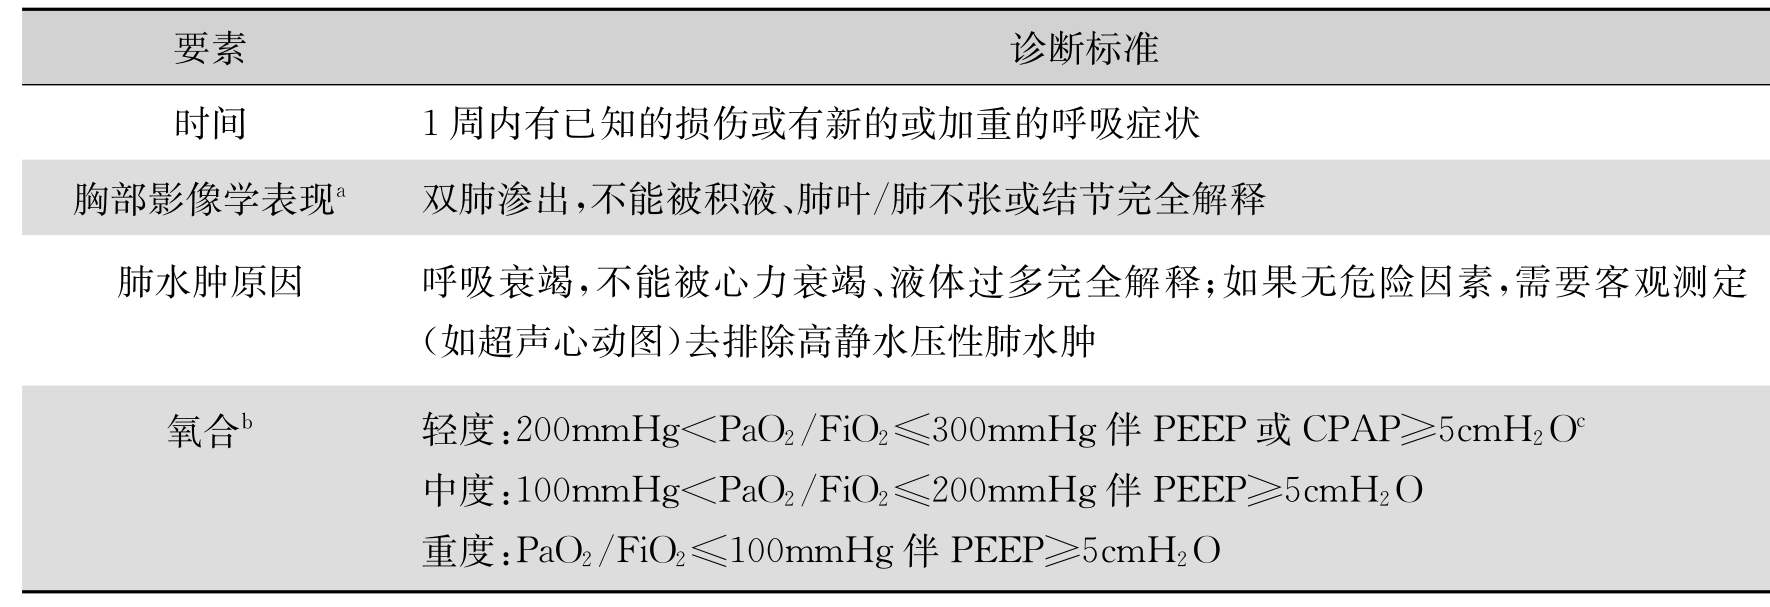
\includegraphics[width=5.89583in,height=2.01042in]{./images/Image00036.jpg}
\end{table}

ARDS诊断时须排除大片肺不张、自发性气胸、上气道阻塞、急性肺栓塞和心源性肺水肿等。与心源性肺水肿的鉴别可根据下列几点:

1.心源性肺水肿的呼吸困难与体位有关,而ARDS则不太明显。

2.心源性肺水肿咳粉红色泡沫样痰,而ARDS的血痰多非泡沫性,而为稀血水样。

3.心源性肺水肿对强心苷、利尿药和血管扩张药有较佳的治疗反应,而ARDS即使吸入高浓度氧疗效不显著。

4.心源性肺水肿湿啰音多集中于肺底,而ARDS的湿啰音分布较广泛,且音调较高,常呈“爆裂音”。

5.心源性肺水肿X线胸片异常阴影与相应的临床表现几乎同时出现,对及时的急救治疗反应常迅速;而ARDS的X线胸片所见疑似肺泡性水肿,但经积极抢救X线征象在数日内无明显好转。鉴别困难时,可通过超声心动图检测心室功能等作出判断并指导此后的治疗。

\paragraph{二、肝肺综合征}

肝肺综合征(HPS)是指肝功能不全引起肺血管扩张、肺气体交换障碍导致的低氧血症及其一系列的病理生理变化和临床表现。常把肝功能不全、肺血管扩张和低氧血症三联症称为HPS。HPS常见于肝炎后肝硬化、酒精性肝硬化及其他原因肝硬化,也可见于慢性活动性肝炎、急性暴发性肝炎、胆汁淤积、非肝硬化性门脉高压(如门体静脉或脾肾静脉吻合手术后)等。国内曾报道两组分别为6例和16例的HPS,均在乙型肝炎、丙型肝炎、酒精性肝病、Wilson病所致的肝硬化基础上发生。

HPS临床上除了肝病的一般表现外,还存在与肝病有关的低氧血症,表现为活动性呼吸困难、发绀、杵状指,其原理是由于肺血管扩张引起的通气/灌注和弥散功能失调。目前认为肺内血管扩张的发生与肺血管扩张物质(如血管活性肠肽等)在肝功能不全时不能被灭活,或经门体分流和淋巴通道进入肺循环,也可能是内皮素、血管紧张素Ⅰ等缩血管物质的缺乏或被抑制,或肺血管内皮细胞对缩血管物质敏感性的下降,致使原关闭的无功能性毛细血管前交通支开放,以及原本正常的低氧性肺血管收缩功能发生障碍。HPS的缺氧表现为直立位低氧,即由卧位改变为直立位时呼吸困难和发绀加剧,PaO\textsubscript{2}
下降10mmHg以上,这是因为肺血管扩张主要位于两肺基底部,直立位时因重力作用影响,流经肺下野的血流量增多,致使肺内右至左分流量增多,氧合障碍进一步加重,缺氧加剧。

确定肺血管扩张是诊断HPS的关键,符合下列条件的可以诊断为HPS:①急、慢性肝脏疾病;②没有原发性心肺疾病,胸片正常或有间质结节状阴影;③肺气体交换异常,有或无低氧血症,P\textsubscript{(A-a}
)O\textsubscript{2}
梯度>15mmHg;④对比增强超声心动描记术(CTTE)及(和)肺灌注扫描,肺血管造影存在肺血管扩张及(或)肺内血管短路;⑤直立位缺氧、气短、发绀,肺骨关节病。诊断标准:肝硬化基础上+微发泡试验阳性+直立位低氧血症(PaO\textsubscript{2}
<70mmHg,即可诊断HPS。如肝硬化基础上+微发泡试验阳性+无直立位低氧血症,说明有肺血管扩张,尚未达到HPS。

\protect\hypertarget{text00047.html}{}{}

\subsection{7.3 胸膜疾病}

\subsubsection{一、自发性气胸}

自发性气胸多以骤然发生的患侧胸痛与呼吸困难起病。严重者(多为张力性气胸)呈进行性呼吸困难、发绀,甚至出现休克。体检发现患侧胸廓饱满,呼吸运动减弱,触觉语颤减弱或消失,叩诊呈鼓音,听诊肺泡呼吸音减弱或消失。气管、心脏与纵隔向健侧移位。临床上一经诊断为张力性自发性气胸,不必等待X线诊断,应立即进行胸腔穿刺排气。

自发性气胸可分成原发性和继发性。继发性发生在有基础肺疾病的患者,由于病变引起细支气管不完全阻塞,形成肺大疱破裂,如肺结核、COPD、肺癌、肺脓肿、尘肺等;原发性发生在无基础肺疾病的健康人,多见于瘦高体型的男性青壮年,常规X线检查肺部无显著病变,但胸膜下可有肺微小疱,多在肺尖部。

根据脏层胸膜破裂情况不同及其发生后对胸腔内压力的影响,自发性气胸通常分为三种临床类型:闭合性(单纯性)、交通性(开放性)及张力性(高压性),见表\ref{tab3-6}。

\begin{table}[htbp]
\centering
\caption{各类型自发性气胸的鉴别}
\label{tab3-6}
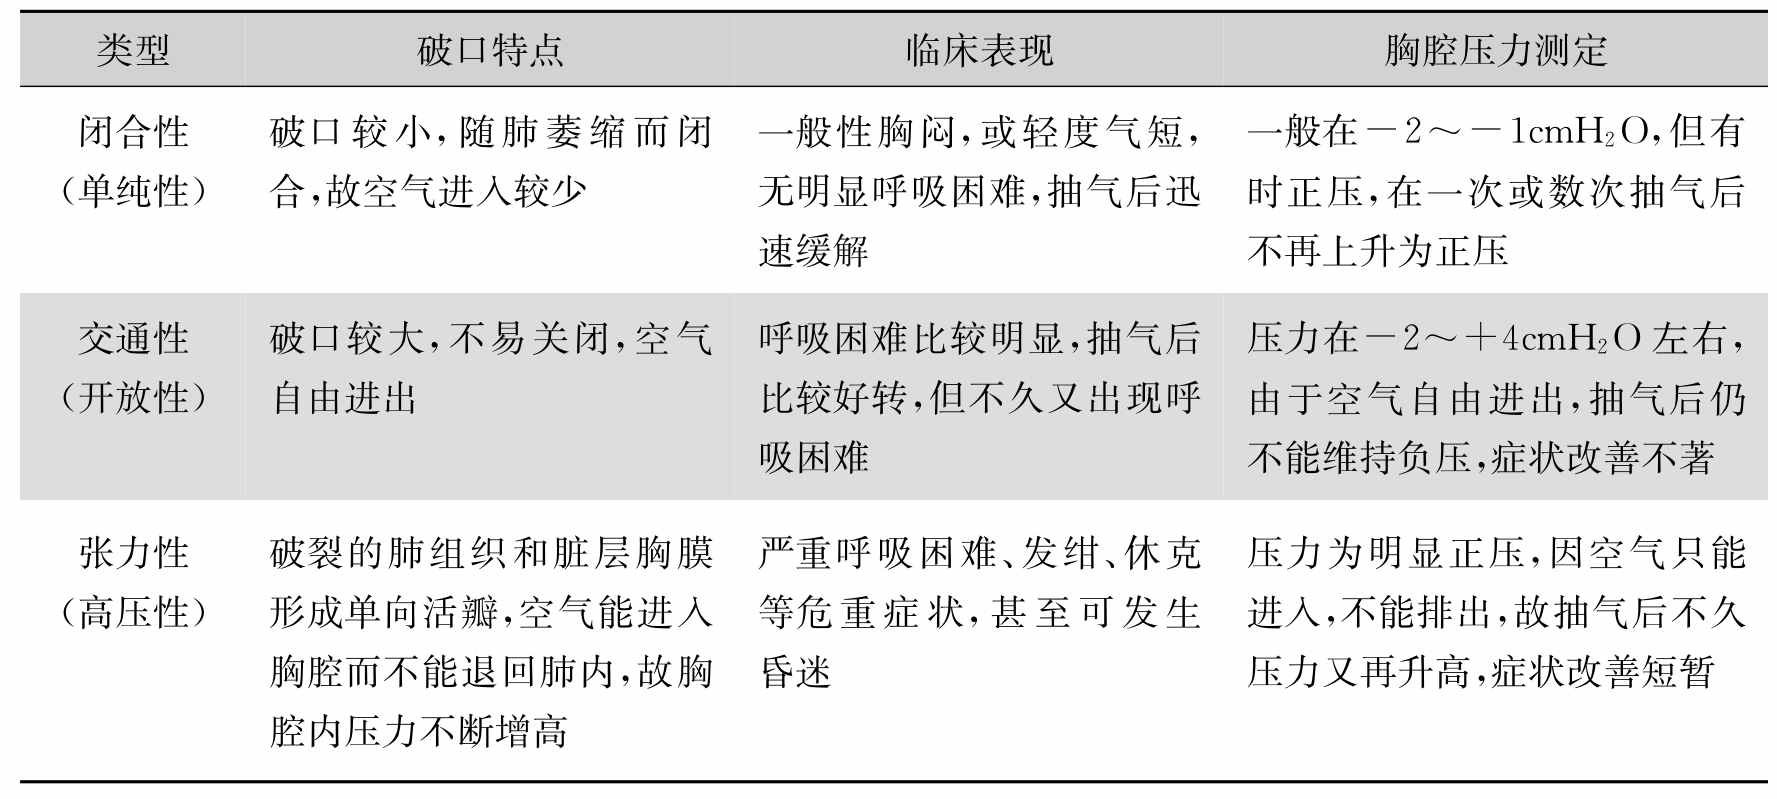
\includegraphics[width=5.91667in,height=2.65625in]{./images/Image00037.jpg}
\end{table}

继发性自发性气胸中最常由肺结核引起,肺结核病灶破裂的特点是:①患者常有发热等结核感染中毒症状;②如有胸腔积液,常为脓性,量常较多;③肺部X线检查通常无肺气肿或肺大疱。

自发性气胸须与肺大疱相区别,主要根据:①后者症状不明显或较轻;②胸部X线检查肺大疱的气腔位于肺实质中,因此在肺尖和肋膈角仍可见有肺组织,并可见气腔内有纤维条索状影像走向肺门,而气胸的气体位于胸腔内,肺组织被推向肺门;③肺大疱有整齐、致密而菲薄的线状泡壁,气腔呈圆形或椭圆形。

\subsubsection{二、大量胸腔积液}

由于大量胸腔积液,压迫肺组织产生压迫性肺不张,使肺呼吸面积减少;同时使纵隔向健侧移位,以致发生呼吸困难。呼吸困难一般发生较缓慢。其严重程度取决于积液产生的速度及其量的大小。急速大量积液时,呼吸困难较明显;积液缓慢发生者,有时可因患者逐渐适应而无呼吸困难。胸腔积液的病因较繁杂(参见第33节)。

\protect\hypertarget{text00048.html}{}{}

\subsection{7.4 纵隔疾病}

\subsubsection{一、急性纵隔炎(参见第33节)。}

\subsubsection{二、慢性纤维性纵隔炎}

慢性纤维性纵隔炎多继发于化脓性或结核性纵隔炎之后,病理改变为纤维组织增生与瘢痕收缩,病变可为广泛性或局限性,症状因纵隔组织受累不同而表现不一。如压迫气管、支气管,则出现气短与呼吸困难;如压迫上腔静脉,则出现上腔静脉阻塞综合征(参见第38节);如压迫喉返神经,则出现声音嘶哑;压迫食管则引起吞咽困难。

\subsubsection{三、纵隔肿瘤及囊肿}

纵隔肿瘤及囊肿发展到一定阶段,压迫或侵犯气管或大支气管时,可引起不同程度的呼吸困难(参见第27.1节)。

\subsubsection{四、纵隔气肿}

严重的纵隔气肿可引起呼吸困难(参见第33节)。

\protect\hypertarget{text00049.html}{}{}

\subsection{7.5 胸廓运动及呼吸肌功能障碍}

胸廓运动受限、呼吸肌和膈肌麻痹、膈高位等皆可使肺呼吸面积减少,而引起呼吸困难。严重的胸廓畸形、肋软骨骨化及硬皮病等均可使胸廓活动受限制;呼吸肌及膈肌麻痹,常由于脊髓灰质炎,脊髓创伤、脑膜炎或脊柱结核所致的神经根病变,多发性神经根神经炎,白喉,重症肌无力等所引起;主动脉瘤可压迫左侧膈神经,肺门部肿瘤或转移瘤也可侵犯膈神经而使膈肌麻痹;膈肌高位常见于妊娠后期、高度的腹水、人工气腹或鼓肠、巨大的腹腔内肿瘤等。

膈肌麻痹

膈肌麻痹分为单侧膈肌麻痹和双侧膈肌麻痹,一般来说单侧膈肌麻痹远多于双侧膈肌麻痹。常见发病原因包括创伤、压力相关、炎症以及神经源性和特发性。其临床表现多种多样,从无症状至呼吸衰竭均可出现,部分患者可表现为重度劳累性呼吸困难以及平卧位呼吸困难,尤其是在夜间快速动眼期可以出现夜间低氧血症和高碳酸血症。因为膈肌麻痹的临床症状无显著特殊性,所以临床上常常误诊为冠状动脉粥样硬化性心脏病、肺炎、肺不张等疾病,据报道平均误诊时间可达2年左右。影像学检查对于诊断膈肌麻痹尤其是单侧膈肌麻痹意义重大,但是对于双侧膈肌麻痹则误诊率高。最大跨膈压检测是诊断膈肌麻痹的金指标。

\protect\hypertarget{text00050.html}{}{}

\subsection{7.6 肺血管病变}

\subsubsection{一、肺栓塞}

肺栓塞和肺梗塞二者有不同的涵义。体循环静脉中或右心的栓子,沿血流进入并堵塞肺动脉或其分支,称为肺栓塞。栓塞部分的肺组织,可因缺氧、坏死而形成肺梗塞。肺栓塞并非都引起肺梗塞。肺梗塞在病理解剖上属于出血性梗塞范畴。

肺栓塞(PE)是以各种栓子阻塞肺动脉系统为其发病原因的一组疾病或临床综合征的总称,包括肺血栓栓塞症(PTE)、脂肪栓塞综合征、羊水栓塞、空气栓塞等。我国由于既往对此病认识不足,临床上经常误诊、漏诊,近年来的研究表明,肺栓塞在我国并非少见。

肺栓塞常见的危险因素和基础病因包括深静脉血栓形成(DVT)、恶性肿瘤、各种心脏病、结缔组织病(系统性红斑狼疮、抗磷脂综合征等)、肾病综合征、外伤、手术和妊娠等。国内一组63例和一组39例的肺栓塞的报道显示最常见的临床症状为呼吸困难、咯血、心悸、胸痛、咳嗽,部分患者有发热、发绀、晕厥等。

\paragraph{(一)肺血栓栓塞症}

PTE为来自静脉系统或右心的血栓阻塞肺动脉或其分支所致的疾病,以肺循环和呼吸功能障碍为其主要临床和病理生理特征。引起PTE的血栓可以来源于下腔静脉径路、上腔静脉径路或右心腔,其中大部分来源于下肢深静脉,特别是从腘静脉上端到髂静脉段的下肢近端深静脉(约占50\%~90\%)。PTE为PE的最常见类型,占PE中的绝大多数,通常所称PE即指PTE。

PTE的临床症状多种多样,均缺乏特异性,症状的严重程度亦有很大差别,可以从无症状到血流动力学不稳定,甚或发生猝死。常见症状包括:呼吸困难及气促、胸痛、晕厥、烦躁不安、惊恐甚至濒死感、咯血、发热等。体检可见呼吸急促、脉速、低血压甚至休克,发绀、颈静脉充盈或搏动、肺部可闻及哮鸣音及(或)细湿啰音,胸腔积液时有相应体征。体检时要注意有否下肢肿胀、压痛、浅静脉扩张、皮肤色素沉着等。

如怀疑PTE,尽快行血浆D-二聚体检测,含量<500mg/L可排除诊断;超声检查可以提示PTE和排除其他疾病;放射性核素肺通气/灌注扫描具有较为重要的诊断或排除诊断意义;螺旋CT、电子束CT或MRI有助于发现肺动脉内血栓的直接证据,已成为临床上经常应用的重要检查手段;肺动脉造影是诊断的“金标准”和参比方法,但为有创性,费用较高。以上检查可根据具体情况选用。

PTE须与急性心肌梗死以及大叶性肺炎相鉴别。急性心肌梗死疼痛多位于心前区,患者有高血压或动脉粥样硬化病史,体温增高较迟于PTE,多在第二、三天才出现,如有咯血与肺局部体征,则更不支持急性心肌梗死的诊断。PTE的典型心电图呈S\textsubscript{Ⅰ}
Q\textsubscript{Ⅲ} T\textsubscript{Ⅲ}
征(即Ⅰ导联S波加深,Ⅲ导联出现Q/q波及T波倒置),往往有完全或不完全性右束支传导阻滞,肺型P波,电轴右偏及顺钟向转位等,如病情好转,心电图改变在较短期间恢复正常,与急性心肌梗死特征性的心电图改变及动态衍变不同,且急性心肌梗死有动态的心肌酶学水平改变。X线检查PTE可发现肺部阴影、肺底浸润或肋膈角模糊阴影,而急性心肌梗死如无发生心力衰竭出现肺水肿则一般没有肺部阴影。大叶性肺炎先有寒战、高热,其后才发生胸痛、咳铁锈色痰,可有唇周疱疹,有典型的胸部X线大叶实变阴影,与PTE不同。

\paragraph{(二)羊水栓塞}

羊水栓塞少见,为一种产科急症,为妊娠期羊水中胎儿产物(胎儿的上皮、毛发、胎脂、黏蛋白、胎粪)进入母体循环而引起。常表现为产妇在破水后不久,突然出现呼吸困难、发绀、抽搐,或兼有休克、昏迷等症状,临床医师应立即考虑此病的可能性,并马上进行诊断与抢救。

发病机制主要由于羊水中胎儿产物作为栓子进入母体循环后可引起肺血管栓塞、变态反应性休克、凝血机制障碍甚至并发弥散性血管内凝血(DIC),影响脏器供血和脏器功能。患者大多数为足月妊娠的中年经产妇,在伴有子宫强烈收缩的情况下发病。由于其发生极其迅速、凶险,病理生理学机制复杂,加之临床医生对它缺乏足够的认识,往往不能及时作出处理,导致母婴死亡率都很高,产妇多因休克、肺水肿或产后大出血而死亡。

肺羊水栓塞有时须与肺血栓栓塞相区别,后者发生于产后静脉血栓形成的基础上,多于产后一周间出现。

\subsubsection{二、肺动脉高压}

肺动脉高压是指孤立的肺动脉血压增高,而肺静脉压力正常,主要原因是肺小动脉原发病变或其他的原发疾病而导致的肺动脉阻力增加,表现为肺动脉压力升高而肺静脉压力在正常范围内,需要肺毛细血管楔压正常才能诊断。肺动脉高压临床表现无特异性,最常见的首发症状是活动后气短、乏力,其他症状有胸痛、咯血、眩晕或晕厥、干咳。气短往往标志肺动脉高压患者出现右心功能不全。而当发生晕厥或眩晕时,则往往标志患者心输出量已经明显下降。查体可见P2亢进;肺动脉瓣开放突然受阻出现收缩早期喷射性喀喇音;三尖瓣关闭不全引起三尖瓣区的收缩期反流杂音;晚期右心功能不全时出现颈静脉充盈或怒张;下肢水肿;发绀;右室充盈压升高可出现颈静脉巨大α波;右室肥厚可导致剑突下出现抬举性搏动;出现S3表示右心室舒张充盈压增高及右心功能不全,约38\%的患者可闻及右室S4奔马律。超声心动图是筛查肺动脉高压最重要的无创性检查方法,可用于估测肺动脉收缩压、评估病情严重程度及预后并协助明确病因。而右心导管检查是确诊肺动脉高压的金标准。

\subsubsection{三、肺静脉堵塞病}

肺静脉堵塞病(pulmonary veno-occlusive
disease,PVOD)是导致肺动脉高压少见的原因之一,它是一种因肺小静脉弥漫性阻塞导致的严重肺动脉高压病,病因目前仍不明确,该病与特发性肺动脉高压临床表现相似,易误诊。目前报道例数较少,对该病的认识不多。床上应用靶向药物治疗反应不佳的肺动脉高压,很可能是被误诊的PVOD,约占最初诊断为特发性肺动脉高压的5\%~10\%。其主要表现为活动后进行性呼吸困难,还有其他症状,如咳嗽、咯血、胸痛、乏力、嗜睡及晕厥等,少数患者可出现弥漫性肺泡内出血和猝死。晚期可出现右心功能不全和右心衰竭的症状和体征,如呼吸频数、发绀、颈静脉怒张、肝颈静脉回流征阳性,心脏听诊P2亢进和三尖瓣反流性杂音,伴有肺部浸润的患者双肺可闻及湿性啰音。此外,PVOD容易合并胸腔积液、心包积液,很少一部分患者也可出现杵状指。胸部影像学特点主要为肺水肿的征象,胸部平片和高分辨率螺旋CT可发现肺充血,Kerley
B线或胸腔积液,肺动脉高压,右心房、右心室扩大,左心房正常等征象。2009年欧洲心脏协会和呼吸协会共同制定该病指南,制定临床诊断标准主要依据:①严重肺动脉高压症状及体征;②胸部影像学提示肺水肿、Kerley
B线或胸腔积液,高分辨CT发现小叶中央毛玻璃样模糊影、间隔线、纵隔淋巴结肿大;③肺动脉楔压(pulmonary
artery wedge
pressure,PAWP)正常或左心房内径正常。符合上述标准可临床诊断为PVOD,不一定需要病理学证据。

\protect\hypertarget{text00051.html}{}{}

\section{8 心源性呼吸困难}

呼吸困难是心功能不全的重要症状之一,其产生的主要原因是:①长期肺淤血,导致肺泡弹性减退,通气功能障碍;②心排血量减少与血流速度减慢,换气功能障碍,导致缺氧与二氧化碳潴留;③肺循环压力增高,导致反射性呼吸中枢兴奋性增高。

心源性呼吸困难的临床特点可概括如下:①患者有重症心脏病存在;②呈混合性呼吸困难,坐位或立位减轻,卧位时加重;③肺底部出现中、小湿啰音;④X线检查心影有异常改变,肺门及其附近充血,或兼有肺水肿征;⑤静脉压正常或升高,臂-舌循环时间延长。

\subsection{一、急性肺水肿}

急性肺水肿的发病主要与肺毛细血管内血压增高、肺毛细血管通透性增加以及血浆胶体渗透压降低等因素有关。主要临床表现是在致病因子的作用下,患者迅速发生胸闷、咳嗽、呼吸困难、发绀和咳出大量白色或浅红色泡沫样痰,并有烦躁不安、大汗、四肢湿冷等症状。听诊双肺弥漫性大、中、小湿啰音。有时可在床边听到“气管沸腾声”。X线胸片检查发现从双侧肺门阴影向外延伸的蝶形阴影。

急性肺水肿的主要原因是:

\subsubsection{1.急性左心衰竭}

如重度二尖瓣狭窄或二尖瓣关闭不全,高血压性心脏病,冠状动脉粥样硬化性心脏病,梅毒性主动脉瓣关闭不全,风湿性主动脉瓣关闭不全或狭窄,急性心肌梗死,嗜铬细胞瘤、急性肾炎或慢性肾炎所致高血压危象等。

\subsubsection{2.肺炎}

如大叶性肺炎、支气管肺炎、重症肺炎等引起中毒性心肌炎。

\subsubsection{3.刺激性气体吸入中毒}

刺激性气体吸入中毒可引起急性肺水肿,其中以二氧化硫、三氧化硫、氯及其化合物、溴甲烷、硫酸二甲酯、光气、氮的氧化物、氢氟酸、氨、硫化氢等较常见。轻者引起上呼吸道刺激征;重者可引起喉水肿、肺炎、肺水肿,导致明显的呼吸困难。肺水肿可突然发生,无前驱症状;但也可逐渐出现。诊断主要根据:①刺激性气体吸入史;②上述的临床表现;③除呼吸道症状外,由于吸入毒物种类的不同,可并发脑、心、肾、肝等器官损害。据此可与其他原因所致的急性肺水肿相区别。

\subsubsection{4.中枢神经系统疾病}

如颅脑外伤、脑炎、脑肿瘤、脑血管意外所致的急性肺水肿。

\subsubsection{5.高原性肺水肿}

国内报告病例大都发生于居留海拔3500~4300米或以上的高原,患者是一向生活于1000米以下的地区,进入高原前未经适应锻炼的人。最短者在进入高原后即发病,最长者可至二年后发病,但大多在进入高原后一个月之内发病。发病大多在冬季,多数与气候突变或大风雪,以及体力劳累有关。前驱症状多有头痛、头晕,继而出现气喘、咳嗽、胸痛,咳大量粉红色泡沫样痰,双肺湿啰音,发绀等表现,严重者出现昏迷。此外皮下水肿、结膜充血、咽充血等也常见。发病机制尚未完全明了。有人认为高原地区大气中氧分压降低、寒冷以及高山适应不全症,三者同时存在为主要的因素。

\subsubsection{6.其他原因}

如输血、输液过量过速,过敏性反应,妊娠中毒症,溺水,烧伤,胸腔穿刺放液过速,有机磷农药中毒等情况,均可引起急性肺水肿。

\subsection{二、充血性心力衰竭}

呼吸困难是充血性心力衰竭的主要症状,且为最早出现的自觉症状。充血性心力衰竭可表现为左心衰竭、右心衰竭或全心衰竭。左、右心衰竭又因病程急慢而区分为急性与慢性。

急性左心衰竭表现为阵发性呼吸困难(心源性哮喘),往往在睡眠中发生,有些患者大脑皮层处于兴奋状态,主诉在噩梦惊醒后即出现,但也可因体力劳动、分娩、精神刺激等而诱发。由于过度的肺淤血而导致急性肺水肿。

慢性左心衰竭常起源于高血压心脏病、二尖瓣膜病、主动脉瓣膜病、冠状动脉粥样硬化性心脏病等。主要症状为呼吸困难、端坐呼吸、发绀、咳嗽、咳血性痰、衰弱、乏力等。体检发现左心增大、心前区器质性杂音、肺动脉瓣第二音亢进、奔马律、双肺底湿啰音等。臂-舌循环时间延长。

左心衰竭持续较长时间的患者通常已有不同程度的右心衰竭。

急性右心衰竭见于肺栓塞所致的急性肺源性心脏病,也可发生于急性风湿性心肌炎、中毒性心肌炎(多表现为全心衰竭,有时以右心衰竭的表现为突出,有时又以左心衰竭较为突出)、重症贫血性或脚气病性心脏病、主动脉窦瘤向右心室穿破等病程中。主要表现为突然出现的呼吸困难、发绀、心动过速、静脉压升高、肝大与压痛、肝颈回流征阳性等。严重病例(如大片肺栓塞)迅速出现休克。但也有报告发生于高原地区。

慢性右心衰竭可起源于慢性肺源性心脏病、某些引起肺动脉狭窄或间隔缺损的先天性心脏病,或由慢性左心衰竭发展而来。患者以慢性体循环淤血为主要表现,出现颈静脉怒张、心悸、气急、发绀、静脉压升高、淤血性肝硬化、蛋白尿、水肿、胸腹积水等症状与体征。也有报告发生于高原地区。

患者具有慢性左心与右心衰竭的征象时,则称为慢性全心衰竭。

\subsection{三、动力不足性心力衰竭}

有人区分心功能不全的另一类型为动力不足性(hypodynamic)心力衰竭,其特征表现是心收缩期异常缩短,心音呈啄木鸟啄击现象(第二心音在第一心音之后迅速出现),心电图上Q-T时间延长,此即心室排血时间的异常缩短,血压正常或降低,X线检查心影无改变。

动力不足性心力衰竭起源于心肌代谢障碍,或心肌收缩过程障碍。此型心力衰竭并非原发性心脏疾病的表现,而常继发于全身性代谢障碍或其他重症全身性疾病,可见于:①各种原因所致的血钾过低;②中毒(如安眠药中毒);③感染(如重症肺炎、白喉、猩红热);④血卟啉病;⑤重症肝功能不全等。

\subsection{四、心包积液}

急性或慢性心包炎(不论何种原因),当心包内产生大量积液时,除了影响心脏的舒张外,可压迫支气管或肺而引起呼吸困难;也可因胸腔积液、肿大的肝脏和大量腹水限制呼吸运动而致呼吸困难。此外,由于心排出量减少,不能满足身体活动的需要,故运动时呼吸困难更为显著。

\protect\hypertarget{text00052.html}{}{}

\section{9 中毒性呼吸困难}

\subsection{一、酸中毒}

各种原因所致的代谢性酸中毒,均可使血液酸碱度(pH)降低,刺激颈动脉窦和主动脉的

化学感受器,或直接兴奋呼吸中枢,增加呼吸通气量与换气量,表现为深而大的呼吸困难。引起代谢性酸中毒的疾病常见于慢性肾炎尿毒症及糖尿病酮症酸中毒或昏迷。临床上发现患者有深而大的呼吸困难而无明显心、肺疾病证据时,须考虑此类疾病的可能性。如患者有广泛性肺部病变而呼吸浅表与发绀时,则须考虑有呼吸性酸中毒的可能性。动脉血气分析可确定诊断。

\subsection{二、化学毒物中毒}

某些毒性物质可作用于血红蛋白,使之失去携氧功能,从而造成组织呼吸(内呼吸)缺氧,出现呼吸困难,临床上常见的有:

\subsubsection{(一)一氧化碳中毒}

一氧化碳进入血液后,与血红蛋白结合成为碳氧血红蛋白,使血红蛋白失去携氧功能致组织缺氧。严重中毒时引起脑水肿与肺水肿。

\subsubsection{(二)氰化物中毒}

氰离子与细胞色素氧化酶中三价铁结合,使之失去传递电子的功能,妨碍细胞的正常呼吸,导致组织缺氧。木薯、苦杏仁含氰化物较多,大量进食后或食用未经去毒处理的木薯而致中毒者也时有见之。电镀、冶炼或生产氰化物过程中,吸入其蒸气或粉尘也是常见的中毒原因。

\subsubsection{(三)亚硝酸盐和苯胺中毒}

亚硝酸盐和苯胺可使血红蛋白转变为高铁血红蛋白,失去携氧能力,而引起呼吸困难(参见第43节)。

\subsubsection{(四)有机磷中毒}

急性有机磷中毒是临床最常见的中毒性疾病之一,患者常出现胸闷、气短、呼吸困难,一般结合患者有机磷接触史、呼出气大蒜味、瞳孔缩小、多汗、肌纤维颤动和意识障碍等,不难作出诊断。如监测血胆碱酯酶活力降低,可确诊。

\subsection{三、药物中毒}

某些中枢抑制剂如吗啡类药物、巴比妥等中毒时,可抑制呼吸中枢,使呼吸慢而浅而出现呼吸困难。

\subsection{四、毒血症}

在急性感染及其他原因的高热时,由于血中毒性代谢产物以及血液温度升高,刺激呼吸中枢,使呼吸增快。

\protect\hypertarget{text00053.html}{}{}

\section{10 血源性呼吸困难}

重症贫血可因血红细胞减少,血氧不足而致气促,尤以劳动后更著。

大出血或休克时,也可因缺血及血压下降,刺激呼吸中枢而引起呼吸困难。

\protect\hypertarget{text00054.html}{}{}

\section{11 神经精神性与肌病性呼吸困难}

重症脑部疾病(如脑炎、脑血管意外、脑肿瘤)直接累及呼吸中枢,可引起呼吸困难,并常出现异常的呼吸节律。

\subsection{(一)中枢神经性换气过度}

是由于中脑下部或桥脑上部的损害所引起,患者常呈木僵或昏迷。呼吸可达100次/分,虽吸入纯氧亦不能使呼吸改善,并可引起呼吸性碱中毒,是严重的临床情况。

\subsection{(二)癔症}

患者可有呼吸困难发作,其特点是呼吸非常频速(一分钟可达80~100次)和表浅,常因换气过度而发生胸痛与呼吸性碱中毒,出现手足搐搦症。诊断须根据病史,并除外器质性病变所致的呼吸困难而确定之。

\subsection{(三)高通气综合征}

可属于心身疾病范畴。国内首次报道的3例均为女性,年龄42~52岁。临床症状累及多器官系统(包括呼吸、循环、神经、精神和心理方面),表现为气短、胸部不适或胸痛、呼吸深大或加快、呼吸困难、心慌或心悸、头昏、视力模糊、手指针刺麻木感、唇周麻木感、晕厥、精神紧张或焦虑、恐惧等。症状可经由过度通气激发试验而复制出来。本综合征须排除器质性疾病,如低氧血症、肺间质纤维化、肺栓塞、代谢性酸中毒、充血性心力衰竭、高热等而确定之。

Nijmegen问卷是目前常用的症状学诊断手段,问卷列举了本征16项常见症状,包括胸痛、精神紧张、视物模糊、头晕、精神错乱或对周围的情况完全不加注意、呼吸深快、气短、胸部发紧或不适、腹胀、手指麻木或针刺感、呼吸困难、手指或上肢强直、口唇周围发绀、手脚冰冷、心悸或心慌、焦虑不安,根据症状出现的频繁程度计分:0=从来没有,1=偶有,2=有时,3=经常,4=频繁。以16项症状总积分≥23作为症状学诊断标准。腹式呼吸训练治疗可成功缓解患者症状,疗效好。根据欧洲不同国家数据表明,本征患者占门诊总人数的4\%~1l\%,好发于女性,25岁以下发病者女性占绝大多数。患者常以胸闷、心前区疼痛或阵发性胸痛等为主诉在心内科诊治,或以失眠、焦虑为主诉就诊于神经内科,易被误诊。

\subsection{(四)重症肌无力危象}

是重症肌无力患者一种极严重的呼吸困难并危及生命的紧急状态。女性发病高峰在30岁左右,男性在50~60岁。诱因最多为上呼吸道感染与肺炎,少数由于分娩、人工流产、胸腺术后、胸腺放射治疗后、应用大剂量泼尼松、注射链霉素、应用巴比妥类药物、停用抗胆碱酯酶剂等。

\protect\hypertarget{text00055.html}{}{}

\section{参考文献}

1.蒋子栋,等.颈段气管相关病变致呼吸困难的诊治.中华医学杂志,2003,83(2):151-152

2.李如竹.急性纤维素性支气管炎.中华内科杂志,1981,20:10

3.顾瑞金.花粉症(附100例报告).中华医学杂志,1964,50:304

4.薛汉麟,等.棉尘肺的观察分析.中华医学杂志,1964,50:389

5.宋仰陶.急性霉蔗尘肺12例临床分析.中华内科杂志,1987,26:356

6.叶世泰.蘑菇肺.中华医学杂志,1981,61:79

7.杨玉.肺嗜酸细胞浸润症54例临床分析.中华内科杂志,1987,26:527

8.彭继繁,等.嗜酸细胞增多性哮喘症455例临床分析.中华内科杂志,1962,10:478

9.张国维,等.吕佛琉氏综合征109例临床X线分析.中华内科杂志,1963,11:822

10.姚应翔.西藏地区高原肺水肿627例临床资料分析.中华内科杂志,1981,20:485

11.蔡柏蔷.100例肺栓塞症临床分析.中华内科杂志,1984,23:253

12.王菊华,等.羊水栓塞.中华妇产科杂志,1979,14(3):206

13.张振磬.重症肌无力危象24例临床分析.中华内科杂志,1982,21:273

14.刘鸿瑞.特发性间质性肺炎的分类和诊断.中华结核和呼吸杂志,2004,27(6):362

15.蔡后荣.2011年特发性肺纤维化诊断和治疗循证新指南解读.中国呼吸与危重监护杂志,2011,10(4):313-316

16.中华医学会呼吸病学分会.特发性肺(间质)纤维化诊断和治疗指南(草案).中华结核和呼吸杂志,2002,25(7):387

17.崔瑷,等.特发性肺纤维化诊治进展:从“专家共识”到以循证医学证据为基础的“诊治指南”.中华医学前沿杂志(电子版),2012,4(1):51-54

18.王振光,等.非特异性间质性肺炎的临床、病理和影像诊断.中华放射学杂志,2004,38(5):543

19.易祥华,等.普通型间质性肺炎的临床病理特征及其与特发性非特异性间质性肺炎的鉴别诊断.中华病理学杂志,2004,33(2):100

20.易祥华,等.非特异性间质性肺炎八例临床病理分析.中华结核和呼吸杂志,2002,25(2):81

21.郭述良,等.变应性肉芽肿性血管炎.中国实用内科杂志,2002,22(6):327-329

22.曾奕明,等.淋巴组织样间质性肺炎二例.中华内科杂志,1998,37(5):346

23.徐作军,等.原发性呼吸道淀粉样变性三例临床分析.中华结核和呼吸杂志,1998,21(12):719

24.何建国,等.全国21家医院急性肺栓塞诊治情况的调查分析.中华医学杂志,2001,81(24):1490

25.蔡柏蔷,等.北京协和医院肺栓塞基础病因的变迁.中华结核和呼吸杂志,2001,24(12):715

26.金英姬,等.肺栓塞39例临床特点分析.中华医学杂志,2003,83(18):1633

27.张红璇,等.肺栓塞诊断及治疗分析.中华急诊医学杂志,2003,12(9):625

28.翟振国,等.肺血栓栓塞症的研究进展.中华结核和呼吸杂志,2004,27(1):14

29.中华医学会呼吸病学分会.肺血栓栓塞症的诊断与治疗指南(草案).中华结核和呼吸杂志,2001,24(5):259

30.中华医学会呼吸病学分会.急性肺损伤/急性呼吸窘迫综合征的诊断标准(草案).中华结核和呼吸杂志,2000,23(4):203

31.刘又宁,等.急性肺损伤/急性呼吸窘迫综合征近年来国内研究进展.中华结核和呼吸杂志,2004,27(1):8

32.苏少慧,等.肝肺综合征16例临床分析,中华结核和呼吸杂志,2002,25(4):251

33.张大志.肝肺综合征的诊断与治疗.中华肝脏病杂志,2009,17(4):256-257

34.韩江娜,等.高通气综合征的临床诊断与治疗.中华结核和呼吸杂志,1998,21(2):98

35.中华医学会呼吸病学分会哮喘学组.支气管哮喘防治指南.中华结核和呼吸杂志,2008,31(3):177-185

36.慢性阻塞性肺疾病诊治指南(2013年修订版).中华医学会呼吸病学分会慢性阻塞性肺疾病学组.中华结核和呼吸杂志,2013,36(4):255-264

37.Raghu G,Collard HR,Egan JJ,et al.An official ATS/ERS/JRS/ALAT
statement:idiopathic pulmonary fibrosis:evidence-based guidelines for
diagnosis and management.Am J Respir Crit Care Med.2011Mar
15;183:788-824

38.ARDS Definition Task Force,Ranieri VM,Rubenfeld GD,Thompson
BT,Ferguson ND,Caldwell E,Fan E,Camporota L,Slutsky AS.Acute
respiratory distress syndrome:the Berlin
Definition.JAMA.2012,307:37:2526-2533

39.急性肺血栓栓塞症诊断治疗中国专家共识.中华医学会心血管病学分会肺血管病学组.中华内科杂志,2010,49(1):74-81

40.Bestall JC,et al.Usefulness of the Medical Research
Council(MRC)dyspnoea scale as a measure of disability in patients with
chronic obstructive pulmonary disease.Thorax.1999;54:581-586

41.Hogan C,et al.Allergic bronchopulmonary aspergillosis and related
allergic syndromes.Semin Respir Crit Care Med.2011,32:682-692

\protect\hypertarget{text00056.html}{}{}

